\documentclass{article}

  % packages
    % basic stuff for rendering math
    \usepackage[letterpaper, top=1in, bottom=1in, left=1in, right=1in]{geometry}
    \usepackage[utf8]{inputenc}
    \usepackage[english]{babel}
    \usepackage{amsmath} 
    \usepackage{amssymb}
    \usepackage{natbib}

    % extra math symbols and utilities
    \usepackage{mathtools}        % for extra stuff like \coloneqq
    \usepackage{mathrsfs}         % for extra stuff like \mathsrc{}
    \usepackage{centernot}        % for the centernot arrow 
    \usepackage{bm}               % for better boldsymbol/mathbf 
    \usepackage{bbm}              % for indicator functions
    \usepackage{enumitem}         % better control over enumerate, itemize
    \usepackage{hyperref}         % for hypertext linking
    \usepackage{xr-hyper}
    \usepackage{fancyvrb}         % for better verbatim environments
    \usepackage{newverbs}         % for texttt{}
    \usepackage{xcolor}           % for colored text 
    \usepackage{listings}         % to include code
    \usepackage{lstautogobble}    % helper package for code
    \usepackage{parcolumns}       % for side by side columns for two column code
    \usepackage{algorithm}
    \usepackage{algpseudocode}

    % page layout
    \usepackage{fancyhdr}         % for headers and footers 
    \usepackage{uniquecounter} 
    \usepackage{lastpage}         % to include last page number in footer 
    \usepackage{parskip}          % for no indentation and space between paragraphs    
    \usepackage[T1]{fontenc}      % to include \textbackslash
    \usepackage{footnote}
    \usepackage{etoolbox}

    % for custom environments
    \usepackage{tcolorbox}        % for better colored boxes in custom environments
    \tcbuselibrary{breakable}     % to allow tcolorboxes to break across pages

    % figures
    \usepackage{pgfplots}
    \pgfplotsset{compat=1.18}
    \usepackage{float}            % for [H] figure placement
    \usepackage{tikz}
    \usepackage{tikz-cd}
    \usepackage{circuitikz}
    \usetikzlibrary{positioning, shapes, arrows, fit, calc}
    \usepackage{graphicx}
    \usepackage{caption} 
    \usepackage{subcaption}
    \captionsetup{font=small}

    % for tabular stuff 
    \usepackage{dcolumn}

    \usepackage[nottoc]{tocbibind}
    \pdfsuppresswarningpagegroup=1
    \hfuzz=5.002pt                % ignore overfull hbox badness warnings below this limit

  % New and replaced operators
    \DeclareMathOperator{\Tr}{Tr}
    \DeclareMathOperator{\Sym}{Sym}
    \DeclareMathOperator{\Span}{span}
    \DeclareMathOperator{\elbo}{ELBO}
    \DeclareMathOperator{\std}{std}
    \DeclareMathOperator{\Cov}{Cov}
    \DeclareMathOperator{\Var}{Var}
    \DeclareMathOperator{\proj}{proj}
    \DeclareMathOperator{\Corr}{Corr}
    \DeclareMathOperator{\pos}{pos}
    \DeclareMathOperator*{\argmin}{\arg\!\min}
    \DeclareMathOperator*{\argmax}{\arg\!\max}
    \newcommand{\ket}[1]{\ensuremath{\left|#1\right\rangle}}
    \newcommand{\bra}[1]{\ensuremath{\left\langle#1\right|}}
    \newcommand{\braket}[2]{\langle #1 | #2 \rangle}
    \newcommand{\qed}{\hfill$\blacksquare$}     % I like QED squares to be black 

  % Custom Environments
    \newtcolorbox[auto counter, number within=section]{question}[1][]
    {
      colframe = orange!25,
      colback  = orange!10,
      coltitle = orange!20!black,  
      breakable, 
      title = \textbf{Question \thetcbcounter ~(#1)}
    }

    \newtcolorbox[auto counter, number within=section]{exercise}[1][]
    {
      colframe = teal!25,
      colback  = teal!10,
      coltitle = teal!20!black,  
      breakable, 
      title = \textbf{Exercise \thetcbcounter ~(#1)}
    }
    \newtcolorbox[auto counter, number within=section]{solution}[1][]
    {
      colframe = violet!25,
      colback  = violet!10,
      coltitle = violet!20!black,  
      breakable, 
      title = \textbf{Solution \thetcbcounter}
    }
    \newtcolorbox[auto counter, number within=section]{lemma}[1][]
    {
      colframe = red!25,
      colback  = red!10,
      coltitle = red!20!black,  
      breakable, 
      title = \textbf{Lemma \thetcbcounter ~(#1)}
    }
    \newtcolorbox[auto counter, number within=section]{theorem}[1][]
    {
      colframe = red!25,
      colback  = red!10,
      coltitle = red!20!black,  
      breakable, 
      title = \textbf{Theorem \thetcbcounter ~(#1)}
    } 
    \newtcolorbox[auto counter, number within=section]{proposition}[1][]
    {
      colframe = red!25,
      colback  = red!10,
      coltitle = red!20!black,  
      breakable, 
      title = \textbf{Proposition \thetcbcounter ~(#1)}
    } 
    \newtcolorbox[auto counter, number within=section]{corollary}[1][]
    {
      colframe = red!25,
      colback  = red!10,
      coltitle = red!20!black,  
      breakable, 
      title = \textbf{Corollary \thetcbcounter ~(#1)}
    } 
    \newtcolorbox[auto counter, number within=section]{proof}[1][]
    {
      colframe = orange!25,
      colback  = orange!10,
      coltitle = orange!20!black,  
      breakable, 
      title = \textbf{Proof. }
    } 
    \newtcolorbox[auto counter, number within=section]{definition}[1][]
    {
      colframe = yellow!25,
      colback  = yellow!10,
      coltitle = yellow!20!black,  
      breakable, 
      title = \textbf{Definition \thetcbcounter ~(#1)}
    } 
    \newtcolorbox[auto counter, number within=section]{example}[1][]
    {
      colframe = blue!25,
      colback  = blue!10,
      coltitle = blue!20!black,  
      breakable, 
      title = \textbf{Example \thetcbcounter ~(#1)}
    } 
    \newtcolorbox[auto counter, number within=section]{code}[1][]
    {
      colframe = green!25,
      colback  = green!10,
      coltitle = green!20!black,  
      breakable, 
      title = \textbf{Code \thetcbcounter ~(#1)}
    } 
    \newtcolorbox[auto counter, number within=section]{algo}[1][]
    {
      colframe = green!25,
      colback  = green!10,
      coltitle = green!20!black,  
      breakable, 
      title = \textbf{Algorithm \thetcbcounter ~(#1)}
    } 
    
    \definecolor{dkgreen}{rgb}{0,0.6,0}
    \definecolor{gray}{rgb}{0.5,0.5,0.5}
    \definecolor{mauve}{rgb}{0.58,0,0.82}
    \definecolor{darkblue}{rgb}{0,0,139}
    \definecolor{lightgray}{gray}{0.93}
    \renewcommand{\algorithmiccomment}[1]{\hfill$\triangleright$\textcolor{blue}{#1}}

    % default options for listings (for code)
    \lstset{
      autogobble,
      frame=ltbr,
      language=Python,                           % the language of the code
      aboveskip=3mm,
      belowskip=3mm,
      showstringspaces=false,
      columns=fullflexible,
      keepspaces=true,
      basicstyle={\small\ttfamily},
      numbers=left,
      firstnumber=1,                        % start line number at 1
      numberstyle=\tiny\color{gray},
      keywordstyle=\color{blue},
      commentstyle=\color{dkgreen},
      stringstyle=\color{mauve},
      backgroundcolor=\color{lightgray}, 
      breaklines=true,                      % break lines
      breakatwhitespace=true,
      tabsize=3, 
      xleftmargin=2em, 
      framexleftmargin=1.5em, 
      stepnumber=1
    }

  % Page style
    \pagestyle{fancy}
    \fancyhead[L]{Factor and Component Analysis}
    \fancyhead[C]{Muchang Bahng}
    \fancyhead[R]{Summer 2025} 
    \fancyfoot[C]{\thepage / \pageref{LastPage}}
    \renewcommand{\footrulewidth}{0.4pt}          % the footer line should be 0.4pt wide
    \renewcommand{\thispagestyle}[1]{}  % needed to include headers in title page

\begin{document}

\title{Factor and Component Analysis}
\author{Muchang Bahng}
\date{Spring 2025}

\maketitle
\tableofcontents
\pagebreak

This covers computability theory, complexity theory, and automata theory. 
Alphabet. Boolean logic


\section{Principal Component Analysis}  

  Say that we have a random vector $x = (x_1, \ldots, x_d)$. These $d$ covariates will naturally be correlated, and we want to ask whether some more fundamental set of independent variables exist \cite{1933hotelling} such that we can express
  \begin{equation}
    x = f(v_1, \ldots, v_k)
  \end{equation} 
  Naturally, we think of $f$ as a linear function. 

  We can think of PCA doing two things. First, it is a dimensionality-reduction algorithm where it takes samples $x \in \mathbb{R}^d$ and projects them into some smaller subspace $\mathcal{L}$ of dimension $k$. Second, it identifies an orthonormal basis of $\mathcal{L}$ that act as uncorrelated low-dimensional features. Because the projection map is linear and we are working in a lower-dimensional subspace, these new basis vectors are linear combinations of the original basis, which may reduce redundancy. Furthermore, by approximately modeling the original $x$ as a linear combination of these features, we are able to get a more parsimonious representation. 

  In PCA literature, it is more common to work with row vectors $x \in \mathbb{R}^{1 \times d}$, so linear mappings are realized through right matrix multiplication $x A$. Furthermore, we will assume that the data are $0$-mean. 

\subsection{L2 Residual Minimization Approach} 

  To give some motivation, we try to find a best fit line in $\mathbb{R}^d$. A line $\ell$ can be parameterized by a unit vector $v$ (note that it can be $-pm v$!), and so given some sample $x$, its projection onto $\ell$ is $\proj_{\ell} (x) = \langle x, v\rangle v$. Therefore, the residual is 
  \begin{align}
    \| x - \langle x, v \rangle v \|^2 & = \|x\|^2 - 2 \langle x, \langle x, v \rangle v \rangle + \| \langle x, v \rangle v \|^2 \\ 
                                       & = \|x\|^2 - 2 \langle x, v \rangle^2 + \langle x, v \rangle^2 \|v\|^2 \\ 
                                       & = \|x\|^2 - \langle x, v \rangle^2
  \end{align}
  since $\|v\|^2 = 1$ \cite{2019shalizi}. Now given a $0$-mean random variable $x$ (why we only consider $0$-mean RVs will be clear later), our risk is
  \begin{equation}
    R(v) = \mathbb{E}_x \big[ \| x - (x \cdot v) v \| \big] = \mathbb{E}_x \big[ \|x\|^2 \big] - \mathbb{E}_x \big[ \langle x, v \rangle^2 \big]
  \end{equation} 

  In practice, we want to minimize our empirical risk. Assume that we have sampled data $x^{(1)}, \ldots, x^{(n)} \sim x$. Then, 
  \begin{align} 
    \argmin_{v \in \mathbb{R}^{d}, \|v\| = 1} \hat{R}(v) 
    & =  \argmin_{v \in \mathbb{R}^{d}, \|v\| = 1} \frac{1}{n} \bigg( \sum_{i = 1}^n \|x^{(i)} \|^2 - \sum_{i=1}^n \langle x^{(i)}, v \rangle^2 \bigg) \\ 
    & = \argmax_{v \in \mathbb{R}^{d}, \|v\| = 1} \frac{1}{n} \sum_{i=1}^n \langle x^{(i)}, v \rangle^2 
  \end{align} 

  We have our loss function! Now what if we wanted to look for best fitting subspaces in general? Let's first rigorously define such a space. 

  \begin{definition}[Principal Subspace] 
    Let $x$ be a $0$-mean random variable in $\mathbb{R}^d$ and let $\mathcal{L}^k$ denote all $k$-dimensional linear subspaces of $\mathbb{R}^d$. The \textbf{$k$th principal subspace} is defined as 
    \begin{equation}
      \ell_k = \argmin_{\ell \in \mathcal{L}_k} \mathbb{E}_{\Tilde{x}} \big[ \| x - \proj_\ell x\|_2 \big]
    \end{equation}
  \end{definition}

  This isn't a big step from what we had before. We just want to construct a subspace $\ell$ that minimizes the expected $L^2$ distance between $x$ and $\ell$. Now how do we do such a thing? The most natural extension would be to identify an orthonormal basis $v_1, \ldots, v_k$, and since 
  \begin{equation}
    \proj_\ell x = \sum_{i=1}^k \proj_{v_i} x
  \end{equation} 
  our loss can be simplified to 
  \begin{align}
    R(\ell) = R(v_1, \ldots, v_k) 
    & = \mathbb{E} \bigg[ \| x - \proj_\ell x \|^2 \bigg] \\ 
    & = \mathbb{E} \bigg[ \|x\|^2 - 2 \langle x, \sum_{i=1}^k \proj_{v_i} x \rangle + \| \sum_{i=1}^k \proj_{v_i} x \|^2 \bigg] \\ 
    & = \mathbb{E} \bigg[ \|x\|^2 - 2 \sum_{i=1}^k \langle x, \proj_{v_i} x \rangle + \sum_{i=1}^k \| \proj_{v_i} x \|^2 \bigg] \\
    & = \mathbb{E} \bigg[ \|x\|^2 - 2 \sum_{i=1}^k \langle x, v_i \rangle^2 + \sum_{i=1}^k \langle x, v_i \rangle^2 \|v_i\|^2 \bigg] \\ 
    & = \mathbb{E} \bigg[ \|x\|^2 - \sum_{i=1}^k \langle x, v_i \rangle^2 \bigg] \label{loss}
  \end{align} 

  Now if $x$ was not $0$-mean, our intuition would tell us that the principal subspace should pass through its mean, or centroid. In fact \cite{1901pearson} showed this for a $1$-dimensional subspace. 

  \begin{lemma}[Principal Subspace Must Intersect Mean]
    Assume that $\mathbb{E}[x] \neq 0$, and by abuse of notation let us denote $\ell + p \in \mathbb{R}^d$ as the affine subspace $\ell$ that goes through $p$ orthogonally from the origin. 

    \begin{figure}[H]
      \centering 
      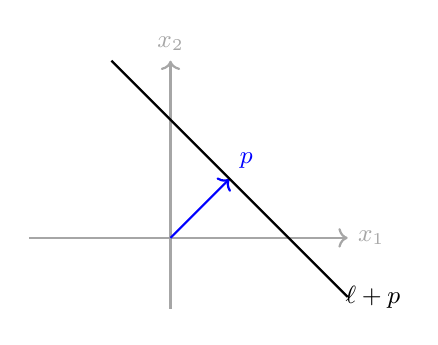
\begin{tikzpicture}[scale=1.5]
        % Axes
        \draw[->, thick, gray!70] (-1.2, 0) -- (1.5, 0) node[right] {\small $x_1$};
        \draw[->, thick, gray!70] (0, -0.6) -- (0, 1.5) node[above] {\small $x_2$};

        % Vector p
        \draw[->, thick, blue] (0,0) -- (0.5, 0.5) node[above right] {\small $p$};

        % Affine subspace l + p (orthogonal to p)
        \draw[thick] (-0.5,1.5) -- (1.5,-0.5);
        \node[] at (1.4,-0.5) [right] {\small $\ell + p$};
      \end{tikzpicture}
      \caption{By orthogonal intersection, we mean that for any $w \in \ell$, $\langle w, p \rangle = 0$} 
    \end{figure}

    Then, we claim that the value of $p$ that minimizes the risk is the average projection distance to the subspace. 
    \begin{equation}
      p = \mathbb{E}[x - \proj_\ell (x)]
    \end{equation}
  \end{lemma}
  \begin{proof}
    The projection distance of $x$ onto $\ell + p$ is the same as the projection distance from $x-p$ onto $\ell$. Therefore, noting that $v_i$'s are orthogonal, we can derive
    \begin{align}
      R(\ell, p) & = \mathbb{E}_x \big[ \| (x - p) - \proj_\ell (x) \|^2 \big] \\
                 & = \mathbb{E}_x \bigg[ \bigg\| (x - p) - \sum_{i=1}^k \proj_{v_i} (x) \bigg\|^2 \bigg] \\ 
                 & = \mathbb{E}_x \bigg[ \|x - p\|^2 + \bigg\| \sum_{i=1}^k \proj_{v_i} (x) \bigg\|^2 - 2 \Big\langle x - p, \sum_{i=1}^k \proj_{v_i} (x) \Big\rangle \bigg] \\ 
                 & = \mathbb{E}_x \bigg[ \|x - p\|^2 - \sum_{i=1}^k \langle x, v_i \rangle^2 + 2 \sum_{i=1}^k \langle x, v_i \rangle \langle p, v_i \rangle \bigg] 
    \end{align}
    To find the minimum, we take the total derivative and set it equal to $0$. We are taking the derivative w.r.t. $p$ of an integral w.r.t. $x$, so we can push the derivative into the integral and solve. 
    \begin{align}
      0 = \frac{\partial R(\ell, p)}{\partial p} 
        &= \mathbb{E}_x \left[ \frac{\partial}{\partial p} \left\{ \|x - p\|^2 - \sum_{i=1}^k \langle x, v_i \rangle^2 + 2 \sum_{i=1}^k \langle x, v_i \rangle \langle p, v_i \rangle \right\} \right] \\
        &= \mathbb{E}_x \left[ 2(p - x) + 2 \sum_{i=1}^k \langle x, v_i \rangle \frac{\partial}{\partial p} \langle p, v_i \rangle \right]  \\ 
        &= \mathbb{E}_x \left[ 2(p - x) + 2 \sum_{i=1}^k \langle x, v_i \rangle v_i \right]  \\ 
        &= \mathbb{E}_x \left[ 2(p - x) + 2 \proj_{\ell} (x) \right]
    \end{align}
    and by solving for $p$, we get 
    \begin{equation}
      p = \mathbb{E}_{x} [x - \proj_\ell (x)]
    \end{equation}
  \end{proof}

  Therefore, we can just normalize the data to $0$ and simply use \ref{loss} without having to account for the affine translation $p$. In the empirical case, we can get rid of the fixed $x$ and find 
  \begin{equation}
    \argmax_{v_i \in \mathbb{R}^d} \frac{1}{n} \sum_{j=1}^n \sum_{i=1}^k \langle x^{(j)}, v_i \rangle^2, \quad \text{ subject to } \|v_i\|^2 = 1, \langle v_i, v_j \rangle = 0 \text{ for } i \neq j
  \end{equation} 

  By stacking the $v_i$'s left-to-right in matrix $V_k \in \mathbb{R}^{d \times k}$, we can get a cleaner form of the loss function. 
  \begin{align}
    \frac{1}{n} \sum_{j=1}^n \sum_{i=1}^k \langle x^{(j)}, v_i \rangle^2 
    & = \frac{1}{n} \sum_{j=1}^n \sum_{i=1}^k (x^{(j)})^T v_i v_i^T x^{(j)} \\ 
    & = \frac{1}{n} \sum_{j=1}^n (x^{(j)})^T V_k V_k^T x^{(j)} \\ 
    & = \frac{1}{n} \Tr(X V_k V_k^T X^T) = \frac{1}{n} \Tr(V_k^T X^T  X V_k) \label{trace}
  \end{align}
  This leads to an intuitive loss function for PCA. 

  \begin{theorem}[Constrained Empirical Risk of $k$th Principal Subspace]
    The empirical risk, or loss function, of PCA is
    \begin{equation}
      \argmax_{V \in \mathbb{R}^{d \times k}, V_k^T V_k = I_k} 
      \frac{1}{n} \| X - X V_k V_k^T\|^2
    \end{equation}
  \end{theorem} 
  \begin{proof}
    By the Frobenius norm expansion and since $V_k^T V_k = I_k$, we have 
    \begin{align}
      \|X - X V_k V_k^T\|_F^2 
      & = \Tr((X - X V_k V_k^T)^T(X - X V_k V_k^T)) \\
      & = \Tr(X^T X - X^T X V_k V_k^T - V_k V_k^T X^T X + V_k V_k^T X^T X V_k V_k^T) \\
      & = \Tr(X^T X) - 2\Tr(X^T X V_k V_k^T) + \Tr(V_k V_k^T X^T X V_k V_k^T) \\ 
      & = \Tr(X^T X) - 2\Tr(V_k^T X^T X V_k) + \Tr(V_k^T V_k V_k^T X^T X V_k) \\
      & = \Tr(X^T X) - 2\Tr(V_k^T X^T X V_k) + \Tr(V_k^T X^T X V_k) \\ 
      & = \Tr(X^T X) - \Tr(V_k^T X^T X V_k) 
    \end{align}
    and since the empirical risk does not depend on $X$, minimizing the Frobenius norm is equivalent to maximizing the second trace term, i.e. \ref{trace}. 
  \end{proof}

  \begin{definition}[Projection Operator]
    Note that there are two distinct projection operators, which are realized through right matrix multiplication. 
    \begin{enumerate}
      \item The linear map $V_k : \mathbb{R}^d \to \mathbb{R}^k$ is a projection operator of the samples $x$ into the component space. 
      \item The linear map $V_k V_k^T : \mathbb{R}^d \to \mathbb{R}^d$ is called the \textbf{rank-k projection operator} onto the $k$th principal subspace. 
    \end{enumerate}
  \end{definition}

  Therefore, $X V_k \in \mathbb{R}^{n \times k}$ is the projection of the dataset into the component space. If we want to get the denoised samples in the sample space $\mathbb{R}^d$, we project it back out $X V_k V_k^T$. 

\subsection{Variance Maximization Approach}

  But we can turn this into a variance maximization problem. Note that $\Var_x [\langle x, v \rangle] = \mathbb{E}_x [ \langle x, v \rangle^2 ] - \mathbb{E}_x [ \langle x, v \rangle]^2$, and so we can rewrite our true risk as 
  \begin{align}
    \argmin_{v \in \mathbb{R}^d, \|v\|=1} R(v) = \argmin_{v \in \mathbb{R}^d, \|v\|=1} \mathbb{E}_x \big[ \|x\|^2 \big] - \Var_x [\langle x, v \rangle] - \mathbb{E}_x [ \langle x, v \rangle]^2
  \end{align} 
  where the last term vanishes since $x$ is $0$-mean, and hence by linearity of expectation $\mathbb{E}_x [\langle x, v \rangle] = \langle \mathbb{E}[x], v \rangle = \langle 0, v \rangle = 0$. In parallel the empirical risk reduces to simply the sample variance. 
  \begin{equation}
    \argmax_{v \in \mathbb{R}^{d}, \|v\| = 1} \hat{\Var}[ \langle x, v \rangle] = \argmax_{v \in \mathbb{R}^{d}, \|v\| = 1} \frac{1}{n} \bigg( \sum_{i=1}^n \langle x^{(i)}, v \rangle^2 \bigg)
  \end{equation} 

  Therefore, we can think of the $L^2$ minimization problem as equivalent to a variance maximization approach.  

  \begin{lemma}[Variance Maximization Approach]
    Minimizing the $L^2$ distance of a random variable $x$ to a line $\ell$ in $\mathbb{R}^d$ is equivalent to maximizing the scalar variance in the projected space. 
    \begin{equation}
      \argmin_{v \in \mathbb{R}^d, \|v\| = 1} \mathbb{E} [ \| x - \proj_v (x) \|_2 ] = \argmax_{v \in \mathbb{R}^d, \|v\| = 1} \Var_x [\langle x, v \rangle ]
    \end{equation}
  \end{lemma}

  \begin{figure}[H]
    \centering
    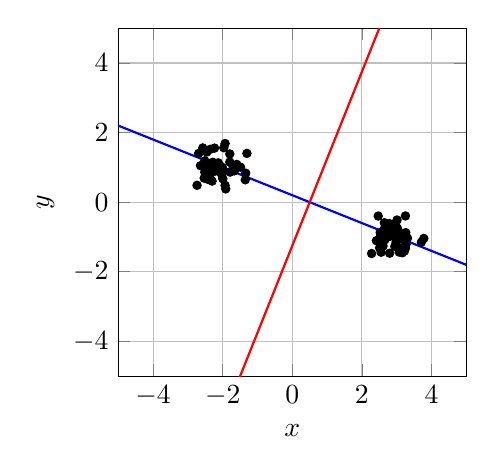
\begin{tikzpicture}
      \begin{axis}[
        xlabel={$x$}, ylabel={$y$},
        axis equal,
        xmin=-5, xmax=5,
        ymin=-5, ymax=5,
        grid=both,
        width=6cm, height=6cm
      ]
      
      \foreach \i in {1,...,50} {
        \pgfmathsetmacro\x{-2 + 0.8*rnd*cos(360*rnd)}
        \pgfmathsetmacro\y{1 + 0.8*rnd*sin(360*rnd)}
        \addplot[only marks, mark=*, mark size=1.5pt, color=black] coordinates {(\x,\y)};
      }
      
      \foreach \i in {1,...,50} {
        \pgfmathsetmacro\x{3 + 0.8*rnd*cos(360*rnd)}
        \pgfmathsetmacro\y{-1 + 0.8*rnd*sin(360*rnd)}
        \addplot[only marks, mark=*, mark size=1.5pt, color=black] coordinates {(\x,\y)};
      }

      % Line from (-2,1) to (3,-1): slope -2/5
      \addplot[thick, blue, domain=-5:5, samples=2] {-0.4*(x + 2) + 1};

      % Perpendicular line through midpoint (0.5, 0), slope 5/2
      \addplot[thick, red, domain=-5:5, samples=2] {2.5*(x - 0.5)};
      \end{axis}
    \end{tikzpicture}
    \caption{Projecting the dataset onto the blue line seems to retain more variance than projecting onto the red line.}
  \end{figure}

  Let's in fact try to directly maximize the variance. If we vertically stack our $n$ data points into a matrix $X \in \mathbb{R}^{n \times d}$, then the projections of this data onto $\mathbb{R}$ is simply $X v \in \mathbb{R}^n$. Again, since this is $0$-mean, the variance is 
  \begin{align}
    \label{eq:var_decom}
    \hat{\Var}(Xv) 
    & = \frac{1}{n} (Xv)^T (Xv) \\ 
    & = \frac{1}{n} v^T X^T X v \\
    & = v^T \frac{X^T X}{n} v \\ 
    & = v^T \hat{\Sigma} v
  \end{align}
  where $\hat{\Sigma}$ is the empirical covariance matrix of $X$. We want to find 
  \begin{equation}
    \max_{v} v^T \hat{\Sigma} v \text{ subject to } \|v\|^2 = 1
  \end{equation} 
  This is a classic Lagrange multiplier problem. We construct the Lagrangian and compute its partial derivatives to set equal to $0$. 
  \begin{align}
    \mathcal{L}(v, \lambda) & = v^T \hat{\Sigma} v - \lambda (\|v\|^2 - 1) \\  
    \frac{\partial \mathcal{L}}{\partial v} & = 2 \hat{\Sigma} v - 2 \lambda v = 0 \\ 
    \frac{\partial \mathcal{L}}{\partial \lambda} & = v^T v - 1 = 0
  \end{align} 
  which gives us 
  \begin{equation}
    \hat{\Sigma} v = \lambda v, \qquad v^T v = 1
  \end{equation} 
  This tells us that $v$ is a unit eigenvector, and the maximizing vector will be the one corresponding to the largest eigenvalue. Essentially, we have reduced this to an eigenvalue problem. 
  
  \begin{theorem}[1st Principal Subspace as Eigenvector]
    The first principal subspace of data matrix $X \in \mathbb{R}^{n \times d}$ is spanned by the eigenvector corresponding to the largest eigenvalue of the sample covariance matrix $\hat{\Sigma} = \frac{1}{n} X^T X$. 
  \end{theorem}

  Now for higher dimensional subspaces, we take the same approach. Going through the same derivation gives the expected risk in terms of the variance 
  \begin{align}
    R(v_1, \ldots, v_k) 
    & = \mathbb{E}[\|x\|^2] - \sum_{i=1}^k \mathbb{E}[ \langle x, v_i \rangle^2 ] \\ 
    & = \mathbb{E}[\|x\|^2] - \sum_{i=1}^k \Var[\langle x, v_i \rangle ] - \mathbb{E}[ \langle x, v_i \rangle ]^2 
  \end{align} 
  By fixing the $x$'s and going through the same derivation as \ref{eq:var_decom}, we get our equivalent empirical risk. 
  \begin{equation}
    \argmax_{v_i \in \mathbb{R}^d} \sum_{i=1}^k \hat{\Var}[\langle x, v_i \rangle] = \argmax_{v_i \in \mathbb{R}^d} \sum_{i=1}^k v_i^T \hat{\Sigma} v_i
  \end{equation}

  \begin{theorem}[Constrained Empirical Risk of $k$th Principal Subspace]
    The empirical risk tells us to find an orthonormal basis that maximizes the sum of the variance of projections. 
    \begin{equation}
      \argmax_{v_i \in \mathbb{R}^d} \sum_{i=1}^k  v_i^T \hat{\Sigma} v_i \text{ subject to } \|v_i\|^2 = 1, \langle v_i, v_j \rangle = 0 \text{ for } i \neq j
    \end{equation}
  \end{theorem}

  The variance-maximization loss is very insightful, and we may naively think of just taking the unit eigenvectors corresponding to the top $k$ largest eigenvalues. Surprisingly, this greedy approach turns out to be correct. 

  Let's derive this further 
  \begin{align}
    \sum_{i = 1}^k v_i^T \hat{\Sigma} v_i 
    & = \sum_{i=1}^k \Tr(v_i v_i^T \hat{\Sigma}) \\ 
    & = \Tr(V_k V_k^T \hat{\Sigma}) \\ 
    & = \Tr(\hat{\Sigma} V_k V_k^T)
  \end{align}
  which again is equal to \ref{trace}. By the spectral theorem, we can take the eigendecomposition of self-adjoint $\hat{\Sigma} = Q \Lambda Q^T$ with orthogonal matrix $Q$. Setting $W_k = Q^T V_k$, we have 
  \begin{equation}
    \Tr(\hat{\Sigma} V_k V_k^T) = \Tr(Q \Lambda Q^T V_k V_k^T) = \Tr(\Lambda Q^T V_k V_k^T Q) = \Tr(\Lambda W_k W_k^T) = \sum_{i = 1}^d \lambda_i (W_k W_k^T)_{ii}
  \end{equation}
  where without loss of generality we have $\lambda_1 \geq \lambda_2 \geq \ldots \geq \lambda_d$. However, we have two constraints. First, since $W_k W_k^T$ is a projection matrix, the eigenvalues must be between $0$ and $1$. Second, by the cyclic trace property, we have $\Tr(W_k W_k^T) = \Tr(I_k) = k$.\footnote{Though it is \textit{not} the case that $W_k W_k^T = I_k$!} So denoting $w_i = (W_k W_k^T)_{ii}$, we have the optimal allocation problem 
  \begin{equation}
    \max \sum_{i=1}^d \lambda_i w_i \text{ subject to } \begin{cases} 
      w_i \in [0, 1] \; \forall i = 1, \ldots, d \\
      \sum_i w_i = k
    \end{cases}
  \end{equation}
  Since the eigenvalues are decreasing, it doesn't take too much to see that the optimal solution is to just put everything you have into the largest eigenvalues. So we fill the first $w_1 = \ldots = w_k = 1$ and the rest $w_{k+1}, \ldots w_d = 0$. Therefore, this solution corresponds to $W_k = (e_1, e_2, \ldots, e_k)$, and so 
  \begin{equation}
    V_k = Q W_k = Q_k
  \end{equation}
  which is the truncated matrix $Q$ containing the first $k$ eigenvectors of $\hat{\Sigma}$ corresponding to the largest eigenvalues. At this point, it does not suffice to talk about just a principal subspace anymore. We must identify its orthonormal basis, i.e. the eigenvectors. 

  \begin{definition}[Principal Axis]
    The eigenvectors $v_1, \ldots, v_k$ that span the $k$th principal subspace are called the top $k$ \textbf{principal axes}, or \textbf{principal directions}.\footnote{The terminology is misused and confusing sometimes. See \href{https://stats.stackexchange.com/questions/88118/what-exactly-is-called-principal-component-in-pca}{https://stats.stackexchange.com/questions/88118/what-exactly-is-called-principal-component-in-pca}.} 
  \end{definition} 
  
  \begin{definition}[Principal Scores]
    Given a sample $x \in \mathbb{R}^d$, its top $k$ \textbf{principal scores} are defined in the equivalent ways. 
    \begin{enumerate}
      \item It is the components of $V_k^T x$. That is, we take a sample and project it onto the component space. 
      \begin{equation}
        x = \sum_i a_i e_i \mapsto V_k^T x = \sum_j b_j e_j^
        \prime
      \end{equation} 
      where $e_i, e_j^\prime$ are the basis vectors in $\mathbb{R}^d, \mathbb{R}^k$. Then $b_1, \ldots, b_k$ are the principal scores of $x$. 

      \item It is the coefficients of $x$ with respect to the basis spanned by the top $k$ eigenvalues. 
      \begin{equation}
        x = c_1 v_1 + c_2 v_2 + \ldots + c_k v_k + c_{k+1} v_{k+1} + \ldots + c_d v_d
      \end{equation} 
      Then $c_1, \ldots, c_k$ are the principal scores. 
    \end{enumerate}
  \end{definition}
  \begin{proof}
    These two are clearly equivalent since 
    \begin{equation}
      b_1 e_1^\prime + \ldots + b_k e_k^\prime = V_k^T x = V_k^T \left( \sum_{i=1}^d c_i v_i \right) = \sum_{i=1}^d c_i V_k^T v_i = \sum_{i=1}^k c_i e_i^\prime 
    \end{equation} 
    which is of the proper form when $c_i = b_i$. Since $V_k^T$ is a truncated orthogonal matrix, $V_k^T v_i = e_i^\prime$ for $1 \leq i \leq k$ and $0$ for all else. 
  \end{proof}

  This is similar to taking the first principal component $v_1$ on $X$, and then by computing the first principal component on the remaining residuals $X - \proj_{v_1} X$, we get the second principal component, which is guaranteed to be orthogonal. But usually, we end up just computing all eigenvectors at once. 

  Now how do we know that this sample decomposition is a good approximation to the true decomposition? It comes from the fact that the sample covariance $\hat{\Sigma}$ is a good approximation of the true covariance $\Sigma$, which we will later prove using concentration of measure. 

  \begin{theorem}[Risk]
    The risk satisfies 
    \begin{equation}
      R(k) = \mathbb{E}[\| x - V_k V_k^T x \|^2 ] = \sum_{j=k+1}^D \lambda_j 
    \end{equation}
  \end{theorem}

  It is essential that you plot the spectrum in decreasing order. This allows you to analyze how well PCA is working. People often use the ``elbow'' technique to determine where to choose $K$, and we value 
  \begin{equation}
    \frac{\sum_{j=1}^k \lambda_j}{\sum_{j=1}^d \lambda_j} 
  \end{equation}
  accounts for the \textbf{variance explained}, which should be high with $K$ low. If you have to go out to dimension $K=50$ to explain $90\%$ of the variance, then PCA is not working. It may not work because of many reasons, such as there being nonlinear structure within the data. 

\subsection{Decomposition Solvers}

  \begin{theorem}[Construction of the kth Principle Subspace] 
    Let $X \in \mathbb{R}^{n \times d}$ be a $0$-mean data matrix. Given the SVD with the singular values listed in decreasing order\footnote{We can make it decreasing by permuting the rows/columns of the unitary matrices $U, V$.}
    \begin{equation}
      X = U \Sigma V^T, \qquad U \in \mathbb{R}^{n \times n}, \Sigma \in \mathbb{R}^{n \times d}, V \in \mathbb{R}^{d \times d}
    \end{equation}
  \end{theorem}

  Since $\frac{1}{n} X^T X = \frac{1}{n} V \Sigma U^T U \sigma V^T = \frac{1}{n} V \Sigma^2 V^T$, the columns of $V$ are the principal axes. Recall from linear algebra that $\Lambda = \Sigma^2$. 

  \begin{algo}[PCA with SVD] 
    Given a dataset $X \in \mathbb{R}^{n \times d}$, let us denote the rows as $x_i$, and say that we are looking for a subspace of dimension $k$. 
    \begin{enumerate}
      \item Compute the mean 
      \begin{equation}
        \mu = \frac{1}{n} \sum_{i=1}^n x_i  \in \mathbb{R}^d
      \end{equation} 

      \item Standardize the data $\Tilde{X} = X - \mu$, i.e. $\Tilde{x}_i = x_i - \mu$.  

      \item Compute the SVD $\Tilde{X} = U \Sigma V^T$.

      \item Compute the submatrices $V_k \in \mathbb{R}^{k \times k}$ and $\Sigma_k \in \mathbb{R}^{D \times k}$. 

      \item Define the projection operator $P_k (x) = \mu + \sum_{j=1}^k \langle x - \mu, v_j \rangle \, v_j$, the change of basis operator $T$, and the embedding operator $T^{-1} (z) = \mu + V_k \Sigma_k z$. 
    \end{enumerate} 
    A demonstration is done \href{code/pca.html}{here}.
  \end{algo}

  \begin{example}[Walkthrough]
    Say that we have some dataset of 100 points in $\mathbb{R}^3$. The data matrix is shown on the right, but in reality I just generated a toy dataset. 

    \noindent\begin{minipage}{.5\textwidth}
      \begin{lstlisting}[]{Code}
        def scatter(n=1000): 
          X_2d = np.random.multivariate_normal(
            np.zeros(2), np.eye(2), n) 
          A = np.array([[1, 1, 1], [-2, 2, 1]])
          X_3d = X_2d @ A + np.random.multivariate_normal(
            np.zeros(3), np.eye(3), n)
          return X_3d
      \end{lstlisting}
      \end{minipage}
      \hfill
      \begin{minipage}{.49\textwidth}
      \begin{lstlisting}[]{Output}
        [[ 8.864e-01  3.975e-01  7.009e-01]
         [-2.065e+00  3.258e+00  1.874e+00]
         [ 3.970e-01 -5.400e-01 -3.054e-01]
         [ 3.239e+00 -1.999e+00 -1.034e+00]
         ...
         [-1.295e-01  9.683e-01  2.861e-01]
         [-7.097e-01 -4.060e-01 -1.058e+00]
         [ 2.284e+00 -2.505e+00 -1.522e+00]]
      \end{lstlisting}
    \end{minipage}

    We can take the SVD, which will give us

    \begin{lstlisting}
      In [7]: U, S, Vt = np.linalg.svd(X)

      In [8]: print(U)
      [[ 4.804e-04  7.852e-02  4.071e-02 ...  5.320e-03  5.034e-02 -9.305e-02]
       [ 1.420e-01  3.992e-02 -1.229e-02 ... -5.512e-02  4.460e-02  7.192e-02]
       [-2.456e-02 -3.657e-03 -4.578e-04 ... -1.005e-01 -1.512e-01 -7.300e-02]
       ...
       [ 2.909e-02  2.754e-02 -1.075e-01 ...  9.871e-01 -1.325e-02 -3.559e-03]
       [-8.714e-03 -8.159e-02 -1.436e-01 ... -1.297e-02  9.733e-01 -1.055e-02]
       [-1.241e-01  2.077e-03 -6.028e-02 ... -3.435e-03 -8.286e-03  9.819e-01]]

      In [9]: print(S)
      [29.90178039 15.17454164  3.01267412]

      In [10]: print(Vt.T)
      [[-0.59855644  0.77282378 -0.21088764]
       [ 0.70716875  0.38606989 -0.59233639]
       [ 0.37635428  0.50367991  0.77760144]] 
    \end{lstlisting} 

    The \texttt{Vt.T} represents $V$, with its columns being our principal axes, and we wish to plot them along with our data points. We would like to scale them by their variance captured. 
    \begin{enumerate}
      \item Take the singular values $(\sigma_1, \sigma_2, \sigma_3) = (29.9, 15.2, 3.0)$. 
      \item Square them to get the eigenvalues $(\lambda_1, \lambda_2, \lambda_3) = (894, 230, 9)$. 
      \item Normalize them to get the percent variance captured. $(0.789, 0.203, 0.008)$, and use this as a scale for each eigenvector. 
    \end{enumerate}

    \begin{figure}[H]
      \centering 
      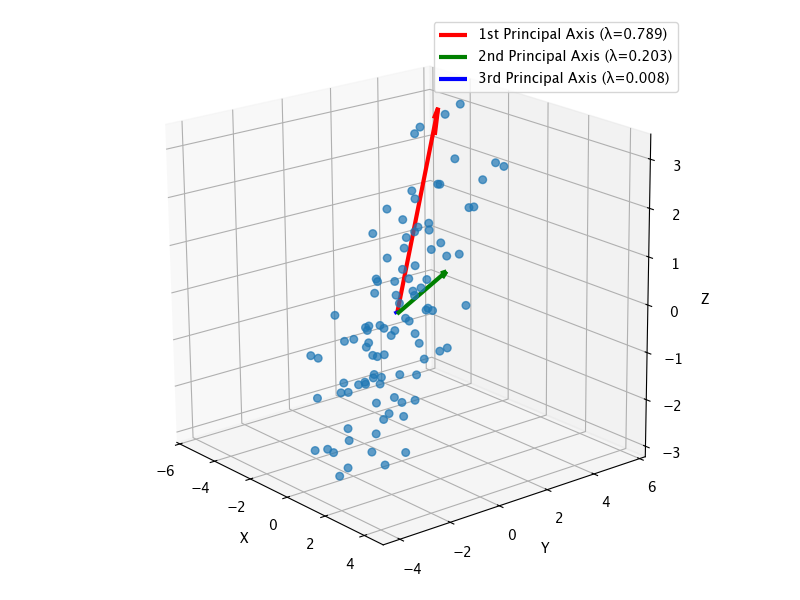
\includegraphics[scale=0.4]{img/pca_3d.png}
      \caption{We can see that the data approximately lies on a 2-dimensional subspace of $\mathbb{R}^3$.} 
    \end{figure}
  \end{example}

  \begin{example}[Eigenfaces]
    In 1991, Turk and Pentland presented an eigenface method of face recognition by taking the low-rank approximation of a dataset of face images \cite{1991turk}. 

    \begin{figure}[H]
      \centering 
      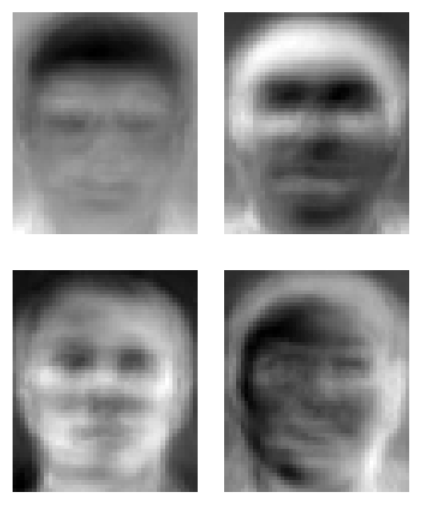
\includegraphics[scale=0.3]{img/eigenfaces.png}
      \caption{Some eigenfaces from AT\&T Labs. } 
      \label{fig:eigenfaces}
    \end{figure}
  \end{example}

\subsection{Iterative Solvers} 

  A disadvantage of decomposition is that the time complexity of SVD on a $n \times m$ matrix is $O(nm \min\{n, m\})$. Therefore, we use iterative methods, which is really just applications of numerical linear algebra. 

\subsubsection{Power Method} 

  The simplest iterative eigenvalue solver was due to von Mises in 1929 \cite{1929vonmises}. Intuitively, given a diagonalizable matrix that we want to solve for, we can  ``normalize'' the spectrum by dividing all the eigenvectors by $\lambda_1$, the largest eigenvalue. Then by composing these linear maps, all the other eigenvectors should die out while keeping the largest eigenvector in place. 

  \begin{theorem}[Convergence of Power Iteration]
    Let $A \in \mathbb{R}^{n \times n}$ be a diagonalizable matrix and $x_0 \in \mathbb{R}^n$ any random vector. Given the two assumptions: 
    \begin{enumerate}
      \item $A$ has a unique greatest eigenvalue $\lambda_1$. 
      \item $x_0$ has a nonzero component in the direction of the eigenvalue $v_1$ associated with $\lambda_1$. 
    \end{enumerate}
    Then, the sequence $(x_t)$ by defined recursively as
    \begin{equation} 
      x_{t+1} = \frac{A x_t}{\|A x_t\|}
    \end{equation}
    converges to $v_1$. 
  \end{theorem}
  \begin{proof}
    We rewrite the recurrence relation as 
    \begin{equation}
    x_{t+1} = \frac{Ax_t}{\|Ax_t\|} = \frac{A^{t+1}x_0}{\|A^{t+1}x_0\|}
    \end{equation}

    Since $A$ is diagonalizable, we can write $A = VSV^{-1}$ where $V$ is the matrix of eigenvectors and $S$ is the diagonal matrix of eigenvalues. Thus:
    \begin{equation}
    x_t = \frac{A^t x_0}{\|A^t x_0\|} = \frac{(VSV^{-1})^t x_0}{\|(VSV^{-1})^t x_0\|} = \frac{VS^t V^{-1} x_0}{\|VS^t V^{-1} x_0\|}
    \end{equation}

    Since $x_0$ can be expressed as a linear combination of eigenvectors, we write $V^{-1}x_0 = c_1 e_1 + c_2 e_2 + \cdots + c_n e_n$ where $e_i$ are the standard basis vectors and $c_i$ are the coefficients. Therefore:
    \begin{align}
      x_t & = \frac{VS^t V^{-1}(c_1 v_1 + c_2 v_2 + \cdots + c_n v_n)}{\|VS^t V^{-1}(c_1 v_1 + c_2 v_2 + \cdots + c_n v_n)\|} \\ 
          & = \frac{VS^t(c_1 e_1 + c_2 e_2 + \cdots + c_n e_n)}{\|VS^t(c_1 e_1 + c_2 e_2 + \cdots + c_n e_n)\|}
    \end{align}

    Factoring out the dominant eigenvalue $\lambda_1$:
    \begin{equation}
      x_t = \left(\frac{\lambda_1}{|\lambda_1|}\right)^t \frac{c_1}{|c_1|} \frac{v_1 + \frac{1}{c_1}V\left(\frac{1}{\lambda_1}S\right)^t(c_2 e_2 + \cdots + c_n e_n)}{\left\|v_1 + \frac{1}{c_1}V\left(\frac{1}{\lambda_1}S\right)^t(c_2 e_2 + \cdots + c_n e_n)\right\|}
    \end{equation}

    Since $|\lambda_i/\lambda_1| < 1$ for $i > 1$, we have $\left(\frac{\lambda_i}{\lambda_1}\right)^t \to 0$ as $t \to \infty$. Therefore:
    \begin{equation}
    \frac{1}{c_1}V\left(\frac{1}{\lambda_1}S\right)^t(c_2 e_2 + \cdots + c_n e_n) \to 0 \text{ as } t \to \infty
    \end{equation}

    Thus, as $t \to \infty$:
    \begin{equation}
    x_t \to \left(\frac{\lambda_1}{|\lambda_1|}\right)^t \frac{c_1}{|c_1|} \frac{v_1}{\|v_1\|} = \pm v_1
    \end{equation}

    Since we assumed that $c_1 \neq 0$, the sequence $(x_t)$ converges to $\pm v_1$. 
  \end{proof}

  Therefore, a direct consequence of this theorem is. 

  \begin{algo}[Power Iteration to Solve Largest Eigenvector]
    Let $A \in \mathbb{R}^{n \times m}$. Then 
    \begin{algorithm}[H]
      \caption{Power Iteration Method}
      \label{alg:power_iteration}
      \begin{algorithmic}[1]
        \Procedure{PowerIteration}{$A$}
            
        \Require{$A \in \mathbb{R}^{n \times n}$ is a matrix, $max\_iter > 0$ is maximum iterations}
        
        \State $x \gets \text{ random vector of unit norm}$
        \State $\lambda \gets 0$
        
        \For{$t \gets 1$ to $max\_iter$}
          \State $y \gets Ax$
          \State $\lambda \gets x^T y$
          \State $x \gets \frac{y}{\|y\|}$
        \EndFor
        
        \State \Return $\lambda, x$
        \EndProcedure
      \end{algorithmic}
    \end{algorithm}
  \end{algo} 

  \begin{corollary}[Rate of Convergence of Power Iteration]
    The rate of convergence is 
    \begin{equation}
      \frac{\lambda_2}{\lambda_1}
    \end{equation}
  \end{corollary}

\subsubsection{Lanczos Algorithms} 

  The time complexity and the slow convergence of the power iteration led to faster algorithms, with one notable class being \textit{Lanczos algorithms}, first developed in 1950 \cite{1950lanczos}. 

  \begin{definition}[Krylov Subspace]
    Given linear map $A: V \to V$ and vector $v \in V$, the \textbf{$m$th Krylov subspace} is 
    \begin{equation}
      \mathcal{K}_m (A, v) = \mathrm{span} \{v, Av, A^2 v, \ldots, A^{m-1} v \}
    \end{equation}
  \end{definition}


  \begin{algo}[Lanczos Algorithm] 
    The basic idea is to construct an orthonormal basis for the Krylov subspace $\mathcal{K}_m (A, v)$ using a three term recurrence relation. This process transforms the original matrix $A$ into a tridiagonal matrix $T$ that can be used to compute the eigenvectors efficiently.  
    
    \begin{algorithm}[H]
      \caption{Lanczos Algorithm}
      \label{alg:lanczos}
      \begin{algorithmic}[1]
        \Procedure{Lanczos}{$A$, $m$}
            
        \Require{Hermitian matrix $A$ of size $n \times n$, number of iterations $m$ (default: $m = n$)}
        \Ensure{$n \times m$ matrix $V$ with orthonormal columns and tridiagonal real symmetric matrix $T = V^* A V$ of size $m \times m$}
        
        \State Let $v_1 \in \mathbb{C}^n$ be an arbitrary vector with Euclidean norm 1
        \State $w_1' \gets A v_1$
        \State $\alpha_1 \gets {w_1'}^* v_1$
        \State $w_1 \gets w_1' - \alpha_1 v_1$
        
        \For{$j \gets 2$ to $m$}
          \State $\beta_j \gets \|w_{j-1}\|$ (Euclidean norm)
          
          \If{$\beta_j \neq 0$}
            \State $v_j \gets w_{j-1} / \beta_j$
          \Else
            \State Pick $v_j$ as arbitrary vector with Euclidean norm 1 orthogonal to all of $v_1, \ldots, v_{j-1}$
          \EndIf
          
          \State $w_j' \gets A v_j - \beta_j v_{j-1}$
          \State $\alpha_j \gets {w_j'}^* v_j$
          \State $w_j \gets w_j' - \alpha_j v_j$
        \EndFor
        
        \State Let $V$ be the matrix with columns $v_1, \ldots, v_m$ and 
        \begin{equation}
          T = \begin{pmatrix}
            \alpha_1 & \beta_2 & & & \\
            \beta_2 & \alpha_2 & \beta_3 & & \\
            & \beta_3 & \alpha_3 & \ddots & \\
            & & \ddots & \ddots & \beta_{m-1} \\
            & & & \beta_{m-1} & \alpha_{m-1} & \beta_m \\
            & & & & \beta_m & \alpha_m
          \end{pmatrix}
        \end{equation}
        
        \State \Return $V, T$
        \EndProcedure
      \end{algorithmic}
    \end{algorithm} 

    For the runtime, 
    \begin{enumerate}
      \item Each iteration consists of an $O(nm)$ matrix multiplication with the rest of the operations $O(n)$. 
      \item If the matrix is sparse, then this is of order $O(nk)$, where $k$ is the average number of nonzero elements in each row. If $k$ is bounded, then we can compute each iteration in linear time $O(n)$. 
    \end{enumerate}
  \end{algo} 

  Now that we have $V, T$, what do we do? The following theorem tells us how to compute the original eigenvectors.  

  \begin{theorem}
    If $\lambda$ is an eigenvalue of $T$ and $x$ is its eigenvector (i.e., $Tx = \lambda x$), then $y = Vx$ is a corresponding eigenvector of $A$ with the same eigenvalue.
  \end{theorem}
  \begin{proof}
    Let $\lambda$ be an eigenvalue of $T$ with eigenvector $x$, so that $Tx = \lambda x$. We need to show that $y = Vx$ is an eigenvector of $A$ with eigenvalue $\lambda$.

    Since the Lanczos algorithm produces the relation $T = V^* A V$, we have $A = VTV^*$. Therefore:
    \begin{align}
      Ay &= AVx \\
         &= VTV^* Vx \\
         &= VTIx \\
         &= VTx \\
         &= V(\lambda x) \\
         &= \lambda Vx \\
         &= \lambda y
    \end{align}
  \end{proof}

  One note of warning. This algorithm tends to be numerically unstable and sometimes there is a loss of orthogonality among the Lanczos vectors due to finite precision arithmetic. We can however just reorthogonalize them in the end. 

\subsubsection{LOBPCG}

\subsubsection{NIPALS}

\subsubsection{Oja's Neuron}

  With neural networks on the rise, Oja developed a simple neuron function that can compute the greatest eigenvector \cite{1982oja}. Let's start with an extremely simple model of a neuron. 

  \begin{definition}[Neuron]
    Consider a linear model of a neuron that returns a sum of its inputs according to weighted presynaptic weights $y(x) = w^T x$. 
  \end{definition} 

  \begin{definition}[Hebb's Rule]
    In neuroscience, \textbf{Hebb's rule} (aka Hebbian learning) colloquially states that neurons are activated together have greater strengths, like how muscles grow when you work them more.\footnote{Neurons that fire together, wire together.}  
    \begin{equation}
      w_{t+1} - w_t = \eta y(x_t) x_t
    \end{equation}
  \end{definition}

  Since the weights are not constrained at all, we would find that the weights approach infinity if $\eta > 0$. Therefore, Oja resticted the weights so that the $p$-norm is $1$ , $0 \leq w_i \leq 1$, which models a form of competition for resources between the neurons \cite{1982oja}. Oja's mathematically formalized this rule in the following. 

  \begin{theorem}[Oja's Rule]
    Hebbian learning of a neuron can be modeled with
    \begin{equation}
      w_{t+1} - w_t = \eta y_t (x_t - y_t w_t)
    \end{equation}
    To parse this, let's focus on a component element $(x_t)_i$. If $x_t$ represents the neurons firing and $y_t w_t$ represents which neurons' wiring scaled by how much the overall neuron has fired, we want the $y_t w_t$ to move closer to $x_t$. Therefore, we update $w_t$ in the direction of this difference, and then scale it by $\eta y_t$. 
  \end{theorem}
  \begin{proof}
    Starting with Hebb's rule and applying normalization constraints, we have\footnote{Oja had $p = 2$ in his original paper, but in fact, any type of normalization, even linear, will give the same result without loss of generality.}
    \begin{equation}
      \mathbf{w}_{t+1} = \frac{\mathbf{w}_t + \eta y_t \mathbf{x}_t}{\left\|\mathbf{w}_t + \eta y_t \mathbf{x}_t\right\|_p}
    \end{equation}
    where $\|\mathbf{v}\|_p = \left(\sum_{j=1}^{m} |v_j|^p\right)^{1/p}$. For a small learning rate $|\eta| \ll 1$, we can expand this equation as a power series in $\eta$. Using the binomial approximation $(1 + \epsilon)^{-1/p} \approx 1 - \frac{\epsilon}{p}$ for small $\epsilon$, we get:
    \begin{equation}
      \mathbf{w}_{t+1} = \frac{\mathbf{w}_t}{\|\mathbf{w}_t\|_p} + \eta \left(\frac{y_t\mathbf{x}_t}{\|\mathbf{w}_t\|_p} - \frac{\mathbf{w}_t \mathbf{w}_t^T \mathbf{x}_t y_t}{\|\mathbf{w}_t\|_p^{p+1}} \|\mathbf{w}_t\|_p^{p-1}\right) + O(\eta^2)
    \end{equation}
   
    For small $\eta$, the higher-order terms $O(\eta^2)$ vanish. We specify a linear neuron where the output is:
    \begin{equation}
      y_t = \mathbf{x}_t^T \mathbf{w}_t^{(p-1)}
    \end{equation}
    where $\mathbf{w}_t^{(p-1)}$ denotes the component-wise power $[\mathbf{w}_t^{(p-1)}]_j = (w_t)_j^{p-1}$. We also specify that our weights are normalized: $\|\mathbf{w}_t\|_p = 1$. 
   
    For $p = 2$, this simplifies to $y_t = \mathbf{x}_t^T \mathbf{w}_t$ and $\|\mathbf{w}_t\|_2 = 1$. Substituting these conditions into our expansion gives:
    \begin{equation}
      \mathbf{w}_{t+1} = \mathbf{w}_t + \eta y_t(\mathbf{x}_t - y_t\mathbf{w}_t)
    \end{equation}
  \end{proof}

  Finally, we claim that $w_t$ asympototically converges to the first principal axes. 

  \begin{theorem}[Oja's Neuron Convergence to First Principal Component]
    Consider a single neuron trained by Oja's rule with weight vector $\mathbf{w}_t$ and input data $\{\mathbf{x}_t\}$ having correlation matrix $R = E[\mathbf{x}\mathbf{x}^T]$. Let $\mathbf{q}_1$ be the eigenvector corresponding to the largest eigenvalue $\lambda_1$ of $R$. Under the following conditions:
    \begin{enumerate}
      \item The learning rate $\eta(t)$ satisfies $\sum_{t=1}^{\infty} \eta(t) = \infty$ and $\sum_{t=1}^{\infty} \eta(t)^p < \infty$ for some $p > 1$
      \item The activation function $y(\mathbf{x}(t))$ is continuously differentiable in both $\mathbf{x}$ and $\mathbf{w}$ with bounded derivatives
      \item The correlation matrix $R$ has a unique largest eigenvalue $\lambda_1$
    \end{enumerate}
    Then the weight vector $\mathbf{w}_t$ converges to $\pm\mathbf{q}_1$ as $t \to \infty$, and the variance of the neuron's output converges to the principal eigenvalue:
    \begin{equation}
      \lim_{t \to \infty} \sigma^2(t) = \lim_{t \to \infty} \langle y^2(t) \rangle = \lambda_1
    \end{equation}
  \end{theorem}
  \begin{proof}
    TBD: Go over this. We analyze the convergence using Lyapunov function analysis. Consider the continuous-time version of Oja's rule:
    \begin{equation}
      \frac{d\mathbf{w}}{dt} = \eta(t) y(t) (\mathbf{x}(t) - y(t) \mathbf{w}(t))
    \end{equation}
    where $y(t) = \mathbf{w}(t)^T \mathbf{x}(t)$.
   
    Taking the expected value and assuming ergodicity of the input process:
    \begin{equation}
      \frac{d\mathbf{w}}{dt} = \eta(t) E[y(\mathbf{x} - y\mathbf{w})] = \eta(t) E[\mathbf{w}^T\mathbf{x}(\mathbf{x} - \mathbf{w}^T\mathbf{x}\mathbf{w})]
    \end{equation}
   
    This simplifies to:
    \begin{equation}
      \frac{d\mathbf{w}}{dt} = \eta(t) (R\mathbf{w} - \mathbf{w}^T R \mathbf{w} \mathbf{w})
    \end{equation}
   
    Since $\mathbf{w}$ is normalized ($\|\mathbf{w}\| = 1$), we have $\mathbf{w}^T R \mathbf{w} = \mathbf{w}^T R \mathbf{w}$. Let $\mathbf{w} = \sum_{i=1}^n c_i \mathbf{q}_i$ where $\{\mathbf{q}_i\}$ are the orthonormal eigenvectors of $R$ with eigenvalues $\{\lambda_i\}$ ordered as $\lambda_1 > \lambda_2 \geq \cdots \geq \lambda_n$.
   
    Substituting the eigendecomposition:
    \begin{equation}
      \frac{d\mathbf{w}}{dt} = \eta(t) \left(\sum_{i=1}^n c_i \lambda_i \mathbf{q}_i - \left(\sum_{i=1}^n c_i^2 \lambda_i\right) \sum_{j=1}^n c_j \mathbf{q}_j\right)
    \end{equation}
   
    For the coefficient $c_1$ corresponding to the first principal component:
    \begin{equation}
      \frac{dc_1}{dt} = \eta(t) c_1 \left(\lambda_1 - \sum_{i=1}^n c_i^2 \lambda_i\right)
    \end{equation}
   
    Since $\lambda_1$ is the largest eigenvalue and $\sum_{i=1}^n c_i^2 = 1$, we have $\lambda_1 - \sum_{i=1}^n c_i^2 \lambda_i > 0$ whenever $c_i \neq 0$ for $i > 1$.
   
    For $i > 1$:
    \begin{equation}
      \frac{dc_i}{dt} = \eta(t) c_i \left(\lambda_i - \sum_{j=1}^n c_j^2 \lambda_j\right)
    \end{equation}
   
    Since $\lambda_i < \lambda_1$, the term $(\lambda_i - \sum_{j=1}^n c_j^2 \lambda_j)$ becomes negative as $c_1$ grows, causing $c_i \to 0$ for $i > 1$.
   
    The conditions on $\eta(t)$ ensure convergence by the Robbins-Monro theorem: the divergent sum condition ensures the algorithm can reach any point in the space, while the convergent power sum condition ensures the noise diminishes sufficiently for convergence.
   
    As $t \to \infty$, we have $c_1 \to \pm 1$ and $c_i \to 0$ for $i > 1$, implying $\mathbf{w}_t \to \pm\mathbf{q}_1$.
   
    The variance of the output is:
    \begin{equation}
      \sigma^2(t) = E[y^2(t)] = E[(\mathbf{w}_t^T \mathbf{x}_t)^2] = \mathbf{w}_t^T R \mathbf{w}_t
    \end{equation}
   
    As $\mathbf{w}_t \to \pm\mathbf{q}_1$, we get:
    \begin{equation}
      \lim_{t \to \infty} \sigma^2(t) = \mathbf{q}_1^T R \mathbf{q}_1 = \lambda_1
    \end{equation}
  \end{proof}
 
  \begin{algo}[Oja's Rule]
    \begin{algorithm}[H]
      \caption{Oja's Neuron Algorithm}
      \label{alg:oja_neuron}
      \begin{algorithmic}[1]
        \Procedure{OjaNeuron}{$\mathbf{x}_1, \mathbf{x}_2, \ldots, \mathbf{x}_T$, $\eta$}
            
        \Require{Input data vectors $\mathbf{x}_t \in \mathbb{R}^n$ for $t = 1, 2, \ldots, T$, learning rate $\eta > 0$}
        \Ensure{Weight vector $\mathbf{w}$ that converges to the first principal component}
        
        \State Initialize $\mathbf{w}_0 \in \mathbb{R}^n$ randomly with small values
        
        \For{$t \gets 1$ to $T$}
          \State $y_t \gets \mathbf{w}_{t-1}^T \mathbf{x}_t$ \Comment{Neural output}
          \State $\mathbf{w}_t \gets \mathbf{w}_{t-1} + \eta y_t (\mathbf{x}_t - y_t \mathbf{w}_{t-1})$ \Comment{Oja's learning rule}
        \EndFor
        
        \State \Return $\mathbf{w}_T$
        \EndProcedure
      \end{algorithmic}
    \end{algorithm}
  \end{algo}

\subsection{The Importance of Standardizing} 

  Say that a covariate was a person's height in meters. If we had measured in centimeters, then the values would a hundred times higher. PCA does not account for this and so in most cases, you should standardize your data to have component-wise unit variance before. 

\subsection{Asymptotic Analysis}

  It turns out that the elements of $\hat{\Sigma}$ are close entry-wise to those of $\Sigma$. But if this is true, then does it mean that the eigenvalues of the sample covariance matrix are close to the true eigenvalues of the covariance matrix? It turns out that the answer is no, and we need a proper metric to satisfy this assumption. The metric, as we can guess from linear algebra, is the operator norm, and we will show some results from matrix perturbation theory. 

  \begin{lemma}[]
    It turns out that 
    \begin{equation}
      ||\hat{\Sigma} - \Sigma|| = O_p \bigg( \frac{1}{\sqrt{n}} \bigg)
    \end{equation}
    where $|| \cdot ||$ is the operator norm. 
  \end{lemma}

  \begin{theorem}[Weyl's Theorem]
    If $\hat{\Sigma}$ and $\Sigma$ are close in the operator norm, then their eigenvalues are close. 
    \begin{equation}
      ||\hat{\Sigma} - \Sigma|| = O_p \bigg( \frac{1}{\sqrt{n}} \bigg) \implies |\hat{\lambda}_j - \lambda_j| = O_p \bigg( \frac{1}{\sqrt{n}} \bigg) 
    \end{equation}
  \end{theorem}

  This only talks about their eigenvalues, but this does not necessarily imply that the eigenvalues are close. We need an extra condition. 

  \begin{theorem}[David-Kahan Theorem]
    If $\hat{\Sigma}$ and $\Sigma$ are close in the operator norm, and if the eigenvectors of $\Sigma$ are well-conditioned, then the eigenvectors of $\hat{\Sigma}$ are close to the eigenvectors of $\Sigma$. More specifically, 
    \begin{equation}
      ||\hat{v}_j - v_j|| \leq \frac{2^{3/2} ||\hat{\Sigma} - \Sigma||}{\lambda_j - \lambda_{j+1}}
    \end{equation}
  \end{theorem}




\section{Factor Analysis} 

  As we have constantly seen, there are specific themes that run between models. In PCA, we have taken some data $x$ in high-dimension $d$ and reduced it to a lower-dimensional orthogonal representation in $\mathbb{R}^k$. In other words, for some sample $x \in \mathbb{R}^{1 \times d}$, the projection onto its component space $x V_k \in \mathbb{R}^{1 \times k}$ is a more parsimonious representation with respect to some other basis vectors. The $v_1, \ldots, v_k$ are new features that are linear combinations of the old vectors. Are they interpretable? In some cases yes and in most cases no, which is why we also call them \textit{latent variables} that live in a \textit{latent space}. 

  Another type of model that encodes covariates in a latent space are factor models, which was developed by Spearman in 1904 \cite{1904spearman}. The general idea was that we have some $d$-dimensional random vector $x$, and we would like to encode it in a $k$-dimensional random vector $f$, called the \textit{factors}. Since we are trying to compress the data, generally $k < d$. The first thing that comes to mind is to try and compare how the variables $x_i$ and $f_j$ correlate to each other, and this is exactly what Spearman did. 

  Before we get into factor models, let's step back and talk more about latent variable models. Colloquially, we would like to find the distribution of some data, whether it'd be $(x, y)$ supervised tasks or $x$ for unsupervised. For the unsupervised case, say that we have some covariates $x$ and we want to find its true distribution $p^\ast$. In density estimation so far, what we have done is define a family of distributions $\{p_\theta\}$ and optimize the loss by maximizing the MLE or something else. 
  \begin{equation}
    \min_\theta L(p_\theta, p^\ast) = \max_\theta \prod_{i} p_\theta(x^{(i)})
  \end{equation}
  In order to do this we work with explicitly parameterized distribution families (e.g. Gaussian, Gamma, multinomial, etc.), but this is too simple to model complex things in real like (e.g. the distribution of faces).

  Therefore, we consider \textit{implicitly parameterized} probability distributions by ``adding'' a latent distribution $z$, creating the joint distribution $(x, z)$. This may look more complicated, but it captures a much richer family of distributions. For example, we might try modeling $x$ as a function of $z$, and try to learn some function $x = f(z)$. If we have an accurate function $f$, we can do many things. 
  \begin{enumerate}
    \item Given an $x$, we might find the closest point on the image of $f$, perhaps some manifold, as low-rank approximation of $x$. This dimensionality reduction is essentially what PCA does with projections.\footnote{We will in fact extend PCA to probabilistic PCA soon to make it generative.} 
    \item If we can sample from $z$, then we can forward it through $f$ and can sample from $x$, making this is a generative model. 
  \end{enumerate}

  Like we do with everything else in math, we take a look at the simplest case when the class of functions are linear. This is known as \textit{linear latent variable modeling}. 
  \begin{equation}
    x = \mu + \Lambda z + \epsilon
  \end{equation}
  where the noise $\epsilon$ is typically Gaussian and diagonal (but not necessarily the same component-wise variances). 

\subsection{Probabilistic PCA}

  We're talking about probabilistic PCA (PPCA), but why is this under factor analysis? I think that the jump from PCA to PPCA is greater than from PPCA to factor analysis, so I will introduce it here as a stepping stone. The main goal of PCA was to do dimensionality reduction by creating a botttleneck in the number of dimensions $k$. Our goal was to approximate the original random variable $x$ by first projecting onto a lower-dimensional space $z = V_k^T x$, and then embedding it through a linear injection. 
  \begin{equation}
    x \approx V_k V_k^T x = V_k z 
  \end{equation} 
  What if we don't restrict the dimensions at all, and just let $k = d$? Then we have the exact equation. 
  \begin{equation}
    x = V V^T x = V z
  \end{equation}
  This is trivial since $V$---as an orthogonal matrix---satisfies $V V^T = V^T V = I_d$. Essentially, this is just a rotation of the axes. We have the maximal restriction when $k = 1$, and as we increase  $k$ to $d$, our reconstruction loss will decrease. But almost always, if our data does not sit exactly on a subspace, we cannot get an exact reconstruction of our data with $k < d$. This is the motivation behind probabilistic PCA (PPCA), and there are essentially two goals that we want to solve. \cite{1999tipping} 
  \begin{enumerate}
    \item \textit{Generative}. We would like our model to be generative. In regular PCA, we saw that for some $z \in \mathbb{R}^k$ in the latent component space, our reconstructed sample is $\hat{x} = S V_k z$. Therefore, if we just change $z$ from a point to a distribution (e.g. Gaussian), we can sample $z \sim \mathcal{N}(0, I_k)$, and then transform it to get a random variable $x = \mu + S V_k z$, which will give a density. 
    \begin{equation}
      x \sim \mathcal{N} \big( \mu, (V_k S)(V_k S)^T \big) = \mathcal{N} \big( \mu, V_k S U^T U S V^T \big) = \mathcal{N} \big( \mu, X_k^T X_k)
    \end{equation} 

    \item \textit{Exact Reconstruction}. However, $X_k \in \mathbb{R}^{n \times d}$ with $d << n$, and so $X_k^T X_k \in \mathbb{R}^{d \times d}$ is not full rank, and so the distribution is restricted to strictly the $k$-dimensional subspace $L_k \subset \mathbb{R}^D$. We want a model that has the both of best worlds: it has a bottleneck so that $k < d$, but at the same time it can do an exact reconstruction of the data. This can be solved by introducing a probabilistic error term $\epsilon$ that accounts for the variability of the data around the principal subspace. So let's add an isotropic Gaussian $\epsilon \sim \mathcal{N}(0, \sigma^2 I)$\footnote{Why isotropic? No real reason. In factor models, we generalize this to arbitrary covariance matrices, and so PPCA is a specific case of factor analysis.}, which gives us 
    \begin{equation}
      x = S V_k z + \epsilon \implies X \sim \mathcal{N}(\mu, X_k^T X_k + \sigma^2 I)
    \end{equation} 
  \end{enumerate} 

  Note again that we are adding \textit{two} probabilistic terms, each of which serves a specific purpose. Great, and finally, let's clean up some notation and polish it up. 
  \begin{enumerate}
    \item First, let's just call $W = S V_k \in \mathbb{R}^{d \times k}$, keeping the $k$ implicit, and treat it as the parameter to estimate. 
    \item Second, let's remove the assumption that $x$ is $0$-mean and add back the mean term $\mu$. 
  \end{enumerate} 

  This gives us our model. 

  \begin{definition}[Probabilistic PCA] 
    The \textbf{probabilistic PCA} model is a latent factor model that summarizes the data generating distribution $x$ as  
    \begin{equation}
      x = \mu + W z + \epsilon, \qquad z \sim N(0, I_k), \epsilon \sim N(0, \sigma^2 I_d) 
    \end{equation} 
    with parameters $\theta = \{\mu, W, \sigma\}$. Let's go over the assumptions. 
    \begin{enumerate}
      \item $z$ is an isotropic Gaussian, which mirrors the fact that the principal components must be orthogonal (uncorrelated RVs). We can normalize it to be unit variance since the scaling can be done with $W$. This allows for a better representation where the components are uncorrelated, and---better yet---we can now sample from $z$. 
      \item $\epsilon$ is an isotropic Gaussian. This is just to ensure that we capture variability beyond the subspace. However, the isotropic part doesn't really seem to be justified... This assumption will be relaxed in factor models.  
    \end{enumerate}
  \end{definition} 

  An immediate consequence is that the closed form of the distrbution of $x$ under this model can be solved. Calculating the pdf of $x$ requires us to marginalize out the $z$, but since marginals of Gaussians are Gaussians, this is quite easy. 

  \begin{lemma}[Likelihood of PPCA] 
    We claim that given $\theta = \{\mu, W, \sigma\}$, we have 
    \begin{equation}
      x \sim \mathcal{N}(\mu, W W^T + \sigma^2 I) 
    \end{equation} 
  \end{lemma}
  \begin{proof}
    By assuming it is Gaussian, you can just directly compute the expectation and covariance, but I will do the full density derivation. We start with the conditional and prior distributions from the probabilistic PCA model:
    \begin{align}
      p(x | z, W) &\propto \exp\left(-\frac{(x - W^T z)^T(x - W^T z)}{2\sigma^2}\right), \\
      p(z) &\propto \exp\left(-\frac{z^T z}{2}\right).
    \end{align}

    The joint distribution is given by:
    \begin{align}
      p(x, z | W) &= p(x | z, W)p(z) \quad \text{(since } z \perp W\text{)} \\
      &\propto \exp\left(-\frac{(x - W^T z)^T(x - W^T z)}{2\sigma^2} - \frac{z^T z}{2}\right).
    \end{align}

    Expanding the quadratic term $(x - W^T z)^T(x - W^T z)$:
    \begin{align}
      (x - W^T z)^T(x - W^T z) &= x^T x - x^T W^T z - z^T W x + z^T W W^T z \\
      &= x^T x - 2x^T W^T z + z^T W W^T z,
    \end{align}
    where we used the fact that $x^T W^T z = z^T W x$ (scalar quantities).

    Substituting back into the joint distribution:
    \begin{align}
      p(x, z | W) &\propto \exp\left(-\frac{x^T x - 2x^T W^T z + z^T W W^T z}{2\sigma^2} - \frac{z^T z}{2}\right) \\
      &= \exp\left(-\frac{x^T x - 2x^T W^T z + z^T W W^T z}{2\sigma^2} - \frac{z^T z}{2}\right).
    \end{align}

    Factoring out $-\frac{1}{2}$ and collecting terms:
    \begin{align}
      p(x, z | W) &\propto \exp\left(-\frac{1}{2}\left(x^T\left(\frac{1}{\sigma^2}I\right)x + 2x^T\left(-\frac{1}{\sigma^2}W^T\right)z + z^T\left(\frac{1}{\sigma^2}WW^T + I\right)z\right)\right).
    \end{align}

    We can rewrite this in quadratic form. Let $v = \begin{bmatrix} x \\ z \end{bmatrix}$. Then:
    \begin{align}
      p(x, z | W) &\propto \exp\left(-\frac{1}{2}\begin{bmatrix} x^T & z^T \end{bmatrix} \begin{bmatrix} \frac{1}{\sigma^2}I & -\frac{1}{\sigma^2}W^T \\ -\frac{1}{\sigma^2}W & \frac{1}{\sigma^2}WW^T + I \end{bmatrix} \begin{bmatrix} x \\ z \end{bmatrix}\right).
    \end{align}

    This has the form of a multivariate Gaussian distribution:
    \begin{equation}
      p(v | W) \propto \exp\left(-\frac{1}{2}(v - \mu)^T\Sigma^{-1}(v - \mu)\right),
    \end{equation}

    with $v = \begin{bmatrix} x \\ z \end{bmatrix}$, $\mu = 0$, and precision matrix:
    \begin{equation}
      \Sigma^{-1} = \begin{bmatrix} \frac{1}{\sigma^2}I & -\frac{1}{\sigma^2}W^T \\ -\frac{1}{\sigma^2}W & \frac{1}{\sigma^2}WW^T + I \end{bmatrix}.
    \end{equation}

    Remember that if we write a multivariate Gaussian in partitioned form,
    \begin{equation}
      \begin{bmatrix} x \\ z \end{bmatrix} \sim \mathcal{N}\left(\begin{bmatrix} \mu_x \\ \mu_z \end{bmatrix}, \begin{bmatrix} \Sigma_{xx} & \Sigma_{xz} \\ \Sigma_{zx} & \Sigma_{zz} \end{bmatrix}\right),
    \end{equation}

    then the marginal distribution $p(x)$ (integrating over $z$) is given by
    \begin{equation}
      x \sim \mathcal{N}(\mu_x, \Sigma_{xx}).
    \end{equation}

    For probabilistic PCA we assume $\mu_x = 0$, but we partitioned $\Sigma^{-1}$ instead of $\Sigma$. To get $\Sigma$ we can use a partitioned matrix inversion formula:
    \begin{equation}
      \Sigma = \begin{bmatrix} \frac{1}{\sigma^2}I & -\frac{1}{\sigma^2}W^T \\ -\frac{1}{\sigma^2}W & \frac{1}{\sigma^2}WW^T + I \end{bmatrix}^{-1} = \begin{bmatrix} W^TW + \sigma^2 I & W^T \\ W & I \end{bmatrix},
    \end{equation}

    which gives that the solution to integrating over $z$ is
    \begin{equation}
      x | W \sim \mathcal{N}(0, W^T W + \sigma^2 I).
    \end{equation}
  \end{proof}

  By taking the log-likelihood, the loss of a single sample is 
  \begin{equation}
    L(x \mid W, \mu, \sigma) = \frac{1}{2} (x - \mu)^T (W^T W + \sigma^2 I)^{-1} (x - \mu)
  \end{equation} 
  and the expected loss is 
  \begin{equation}
    \mathbb{E}_x [ L(x \mid W, \mu, \sigma)] = \int L(x \mid W, \mu, \sigma) \, p(x) \,dx
  \end{equation}
  Likewise, the empirical loss for a dataset of $n$ elements $\{x^{(i)}\}_{i=1}^n$ is 
  \begin{equation}
    \frac{1}{2} \sum_{i=1}^n (x^{(i)} - \mu)^T (W^T W + \sigma^2 I)^{-1} (x^{(i)} - \mu)
  \end{equation}

  Optimizing this model is actually quite easy. 


  \begin{theorem}[MLE of PPCA Model]
    Given $x^{(i)} \sim X$ iid, the MLEs for $W, \mu, \sigma$ are 
    \begin{align}
      \mu^\ast & = \frac{1}{n} \sum_{i=1}^n x^{(i)} \\
      \sigma^{2 \ast} & = \frac{1}{d-k} \sum_{j=k+1}^d \lambda_j \\
      W^\ast & = R (\hat{\Sigma} - \sigma^{2 \ast} I_d )^{1/2} V_k
    \end{align}
    where $\lambda_j$ are the eigenvalues of $X^T X$ in decreasing order, $V_k$ is the truncated orthogonal matrix consisting of the first $k$ columns of $V$ for SVD $X = U S V^T$, and $R$ is any unitary matrix.\footnote{Note that $W^{\ast}$ is not unique. Say that $W^\ast$ is an MLE, then, for any unitary $R \in \mathbb{R}^{d \times d}$, we have $W^{\ast T} W^\ast = (R W^\ast)^T (R W^\ast)$.} 
  \end{theorem}
  \begin{proof}
    We could also just differentiate the expected risk directly, but for no particular reason I will differentiate the empirical risk. 
    \begin{enumerate}
      \item For $\mu^\ast$, we use the matrix derivative $\frac{\partial}{\partial x} x^T A x = 2 A x$ and get 
      \begin{align}
        0 & = \frac{1}{2} \sum_{i=1}^n \frac{\partial}{\partial \mu} \left\{ (x^{(i)} - \mu)^T (W^T W + \sigma^2 I) (x^{(i)} - \mu) \right\} \\ 
          & = \frac{1}{2} \sum_{i=1}^n 2 (W^T W + \sigma^2 I) (x^{(i)} - \mu) \\ 
          & = (W^T W + \sigma^2 I) \left( \sum_{i=1}^n x^{(i)} - \mu \right)
      \end{align} 
      and since $W^T W + \sigma^2 I$ is positive definite, its inverse is positive definite and so it can only be $0$ when it is mapping the $0$ vector. So $\mu = \sum_{i=1}^n x^{(i)}$. 

      \item For $\sigma$, we first take a look at $C = \mathrm{Var}[X] = W W^T + \sigma^2 I$. It is the sum of positive semidefinite matrices that are also symmetric, so by the spectral theorem it is diagonalizable and has full rank $d$. But $W W^T$ is rank $k$, so $d - k$ of the eigenvalues of $W W^T$ is $0$, indicating that the same $d-k$ smallest eigenvalues of $C$ is $\sigma^2$. Therefore, we can take the smallest $d-k$ eigenvalues of our MLE estimator of $C$ and average them to get our MLE for $\sigma$. 
      \begin{equation}
        \hat{\sigma}^{2\ast} = \frac{1}{d-k} \sum_{j=k+1}^d \lambda_j
      \end{equation}
      \item TBD: Justify this again. For $W$, we can set $\mu^\ast$ first and then compute 
      \begin{equation}
        \widehat{\mathrm{Var}}(\mu^{\ast}) = \hat{\Sigma} = \frac{1}{n} \sum_{i=1}^n (x^{(i)} - \mu^{\ast}) (x^{(i)} - \mu^{\ast})^T
      \end{equation}
      We can approximate $W W^T = C - \sigma^2 I \approx \hat{\Sigma} - \hat{\sigma}^{2\ast} I$, and by further taking the eigendecomposition $C = U \Sigma U^T \implies W W^T = U (\Sigma - \sigma^2 I) U^T$ and cutting off the last $d-k$ smallest eigenvalues and their corresponding eigenvectors, we can get 
      \begin{equation}
        W^{\ast} = R (\Sigma - \sigma^{2 \ast} I_d )^{1/2} V_k
      \end{equation}
      where the $R$ just accounts for any unitary matrix. 
    \end{enumerate}
  \end{proof}

  It turns out that the MLE of $W$ for PPCA, denoted $W_{\mathrm{PPCA}}^\ast = (\Sigma - \sigma^{\ast 2} I_d)^{1/2} V_k$ has columns in the same direction but with a smaller length than $W_{\mathrm{PCA}} = S V_k = \Sigma^{1/2} V_k$ for standard PCA. For this reason, you should think of PPCA as ``almost'' PCA. 

  Our next result is intuitive. We have introduced the error term $\epsilon$ that allows us to extend beyond the principal subspace. If we let $\epsilon$ vanish, the density model defined by PPCA becomes very sharp around these $d$ dimensions spanned by the columns of $W$. At $0$, we are reduced to regular PCA. 

  \begin{theorem}[PPCA as $\sigma \to 0$] 
    As $\sigma \rightarrow 0$, the MLE estimates of $W$ is equivalent to that of PCA. That is, when $W \in \mathbb{R}^{d \times k}$, 
    \begin{equation}
      W^\ast = \Sigma V_k
    \end{equation} 
    where $X = U \Sigma V^T$, and $V_k$ is the matrix formed by the first $k$ columns of $V$. That is, the conditional expected value of $z$ given $X$ becomes an orthogonal projection of $X - \mu$ onto the subspace spanned by the columns of $W$. 
  \end{theorem}
  \begin{proof}
    At $0$, our MLE of $W$ is simplified and we have 
    \begin{equation}
      x = W^\ast z + \mu^\ast + \epsilon = \Sigma V_k z + \mu^\ast
    \end{equation}
    which essentially reduces to regular PCA. 
  \end{proof}

  Intuitively, we can see that we are estimating the Gaussian, which corresponds to the mean squared distance from each $x^{(i)}$ to $\ell_k$. 

\subsection{Linear Factor Models} 

  A linear factor model is pretty much the same thing as PPCA. In fact, I don't even know why these two models are distinguished. The only two differences is notation and that linear factor models loosen the restriction that the covariance matrix of $\epsilon$ must be isotopic. 

  \begin{definition}[Factor Analysis] 
    A \textbf{linear factor model} is a latent factor model that models the data generating distribution $x$ over $\mathbb{R}^d$ as 
    \begin{equation}
      x = \mu + \Lambda \eta + \epsilon, \eta \sim N(0, I_k), \epsilon \sim N(0, \Psi)
    \end{equation}
    for some diagonal matrix $\Psi$. The parameters are $\theta = \{\Lambda, \mu, \Psi\}$.\footnote{It is also common notation to use $L$ and $f$ as the loading matrix and factors.} Let's go over the assumptions. 
    \begin{enumerate}
      \item $\mu = \mathbb{E}[x]$ simply normalizes the distribution. 
      \item $\eta \in \mathbb{R}^k$ are the \textbf{factors} that act as latent variables. It is $0$-mean (since the translation is captured in $\mu$) and isotropic, which parallels the uncorrelated assumptions of PCA and PPCA. 
      \item $\Lambda \in \mathbb{R}^{d \times k}$ is the \textbf{loading matrix} that maps the factors to the samples. 
      \item $\epsilon$ is an error term, assumed to be isotropic, and the component variables must be uncorrelated. 
      \item The noise $\epsilon$ is uncorrelated with $\eta$. 
    \end{enumerate}
  \end{definition} 

  The biggest glaring change is really just the terminology. Rather than components, we say \textit{factors}, and rather than projections, we say \textit{loadings}. Finally, we say observable component $x_i$ \textit{loads on} factor $z_j$ if $\Lambda_{ji} \neq 0$, i.e. if $z_j$ affects the value of $x_i$. 

  However, factor models just have more degrees of freedom. In practice, they also perform very similarly. 

  To get more comfortable with the notation, let's write out the formula given a data matrix. If we were working with the data matrix $X \in \mathbb{R}^{n \times d}$, then we would be using right matrix multiplication, and so our model will look like 
  \begin{equation}
    X - \mu = \eta \Lambda + \epsilon
  \end{equation}
  where $\eta \in \mathbb{R}^{n \times k}$, $\Lambda \in \mathbb{R}^{k \times d}, \epsilon \in \mathbb{R}^{n \times d}$. 

  \begin{lemma}[Likelihood of Linear Factor Models]
    The likelihood of the linear factor model is 
    \begin{equation}
      x \sim \mathcal{N}(\mu, W W^T + \Psi)
    \end{equation}
  \end{lemma}
  \begin{proof}
    It should be clear to us that $X$ should be Gaussian since linear transformations of Gaussians are Gaussian. Therefore it suffices to compute its mean and variance. 
    \begin{enumerate}
      \item The mean can be computed exactly the same way for PPCA, which gives $\mathbb{E}[X] = \mu$. 
      \item The variance can be computed as 
      \begin{align} 
        \mathrm{Var}[X] & = \mathbb{E}[ (X - \mu)(X - \mu)^T ] \\
                        & = \mathbb{E}[ (W Z + \epsilon) (Z^T W^T + \epsilon^T)] \\
                        & = \mathbb{E}[W z z^T W^T] + \mathbb{E}[ \epsilon \epsilon^T] \\
                        & = W \mathbb{E}[ z z^T] W^T + \mathbb{E}[ \epsilon \epsilon^T] \\
                        & = W W^T + \Psi
      \end{align} 
    \end{enumerate}
  \end{proof}

  The $W, \mu$, and $\sigma_i$'s can be estimated using MLE methods. The solutions are very similar to that of PCA, with non-uniqueness of $W$ up to rotational factor. 

  \begin{theorem}[MLE of Factor Model]
    Given $x^{(i)} \sim X$ iid, the MLEs for $W, \mu, \Psi$ are 
    \begin{align}
      \mu^\ast & = \frac{1}{n} \sum_{i=1}^n x^{(i)} \\
      \Psi^\ast & = \\
      W^\ast & = R (\Sigma - \sigma^{2 \ast} I_d )^{1/2} V_k
    \end{align}
    where $\lambda_j$ are the eigenvalues of $X^T X$ in decreasing order, $V_k$ is the truncated orthogonal matrix consisting of the first $k$ columns of $V$ for SVD $X = U \Sigma V^T$, and $R$ is any unitary matrix.\footnote{Note that $W^{\ast}$ is not unique. Say that $W^\ast$ is an MLE, then, for any unitary $R \in \mathbb{R}^{d \times d}$, we have $W^{\ast T} W^\ast = (R W^\ast)^T (R W^\ast)$.} 
  \end{theorem}

\subsection{Numerical Solvers for Linear Factor Models}
  
  There is not an analytical solution of factor models. So there is no Eckart-Young theorem that gives a nice decomposition approach to solve factor models. Therefore, we must resort to numerical techniques. 

\subsubsection{Iterated Principal Factors}

  \begin{algo}[Iterated Principal Factors]
    
  \end{algo}

\subsection{PCA vs PPCA vs Factor Models} 

  We have stressed that FA is the same as PPCA, but let's get serious and talk about the differences. In a sense, we could have reformulated PCA as a probabilistic model by assuming that the error terms were normally distributed with variance \textit{orthogonal} to the principal subspace. This would have given the exact same expected risk and thus the models would be equivalent. On the other hand, probabilistic PCA assumes an isotropic Gaussian and factor models assume uncorrelated Gaussian. 

  \begin{figure}[H]
    \centering
    \begin{subfigure}[b]{0.6\textwidth}
      \centering
      
\begin{tikzpicture}[scale=1.5]
        % Left: Green diagonal line through cross
        \draw[thick] (-0.8, 0) -- (0.8, 0);  % horizontal
        \draw[thick] (0, -0.8) -- (0, 0.8);  % vertical
        \draw[thick, green!70!black, line width=2pt] (-0.6, -0.6) -- (0.6, 0.6);  % diagonal
        
        % Right: Plus sign and yellow diagonal
        \node at (1.5, 0) {$+$};
        \draw[thick] (2.2, 0) -- (3.8, 0);   % horizontal
        \draw[thick] (3, -0.8) -- (3, 0.8);  % vertical
        \draw[thick, orange!80!yellow, line width=2pt] (2.4, 0.6) -- (3.6, -0.6);  % diagonal
      \end{tikzpicture}
      \caption{Probabilistic interpretation of regular PCA.}
    \end{subfigure}
    
    \begin{subfigure}[b]{0.6\textwidth}
      \centering
      
\begin{tikzpicture}[scale=1.5]
        % Left: Green diagonal line through cross (same as top)
        \draw[thick] (-0.8, 0) -- (0.8, 0);  % horizontal
        \draw[thick] (0, -0.8) -- (0, 0.8);  % vertical
        \draw[thick, green!70!black, line width=2pt] (-0.6, -0.6) -- (0.6, 0.6);  % diagonal
        
        % Right: Plus sign and yellow circle
        \node at (1.5, 0) {$+$};
        \draw[thick] (2.2, 0) -- (3.8, 0);   % horizontal
        \draw[thick] (3, -0.8) -- (3, 0.8);  % vertical
        \draw[thick, orange!80!yellow, line width=2pt] (3, 0) circle (0.5);  % circle
      \end{tikzpicture}
      \caption{Regular interpretation of probabilistic PCA.}
    \end{subfigure}
    
    \begin{subfigure}[b]{0.6\textwidth}
      \centering
      
\begin{tikzpicture}[scale=1.5]
        % Left: Green diagonal line through cross (same as second)
        \draw[thick] (-0.8, 0) -- (0.8, 0);  % horizontal
        \draw[thick] (0, -0.8) -- (0, 0.8);  % vertical
        \draw[thick, green!70!black, line width=2pt] (-0.6, -0.6) -- (0.6, 0.6);  % diagonal
        
        % Right: Plus sign and yellow circle
        \node at (1.5, 0) {$+$};
        \draw[thick] (2.2, 0) -- (3.8, 0);   % horizontal
        \draw[thick] (3, -0.8) -- (3, 0.8);  % vertical
        \draw[thick, orange!80!yellow, line width=2pt] (3, 0) ellipse (0.7 and 0.4);  % ellipsoid
      \end{tikzpicture}
      \caption{Factor analysis.}
    \end{subfigure}
    \caption{The green (left) represents the latent feature, and the orange on the right represents the errors. Figure credits to \textit{ttnphns} from \href{https://stats.stackexchange.com/questions/1576/what-are-the-differences-between-factor-analysis-and-principal-component-analysi}{here}.}
  \end{figure}

  It turns out that this simple change of not having constant variance in the Gaussian error term $\epsilon$ has some implications. 

  \begin{example}[Scaling Features does not Affect FA]
    Remember that in PCA, we must normalize each component of the data to unit variance since PCA tries to maximize variance of projections. However, FA does not chase large-noise features that are uncorrelated with other features. 
  \end{example}

  \begin{example}[FA is Affected by Rotation of Data]
    FA is affected by rotation of the data. \cite{2018schmidt}
  \end{example}

  \begin{theorem}[Factor Models Converge to PPCA in High Dimensions]
    As $d \to +\infty$, factor models are the same model as PPCA. 
  \end{theorem}



\section{Robust PCA}

\section{Sparse PCA}


\section{Dynamic PCA}

\section{Functional PCA}

\section{Kernel PCA}

  \begin{definition}[Kernel PCA]
    Let $N_i$ be the neighborhood around $X_i$. Then, we want to find a mapping $W: \mathbb{R}^n \rightarrow \mathbb{R}^k$ that minimizes 
    \begin{equation}
      \min_{W} \sum_{i=1}^n \bigg| \bigg| X_i - \sum_{j \in N_i} W_{ij} X_j \bigg| \bigg|^2 \text{ where } \sum_{j} W_{ij} = 1
    \end{equation}
    We can constrain the weights in $W$ so that anything that is not in the neighborhoods are $0$. 
  \end{definition}


\section{Group PCA}


\section{Probabilistic PCA}

  \begin{definition}[Generative Latent Variable Model]
    A \textbf{latent variable model} is a model of a distribution $p^\ast (x)$ over a space $\mathcal{X}$ using implicitly parameterized probability distributions $p_\theta$ constructed as such: 
    \begin{enumerate}
      \item We define a simple random variable $Z$ over $\mathcal{Z}$ with its distribution $p(z)$, called the \textbf{prior}.\footnote{Almost always a uniform or normal distribution suffices. If not, we can constrain it to be factorable (i.e. is the product of its marginal distributions: $p(z) = \prod_i p(z_i)$) so that it is easy to sample from. Occasionally, the stronger assumption of the $z_i$'s being iid is made. } 
      \item We define a family of functions $\{f_\theta\}$ defined over $z$ and parameterized by $\theta$. 
      \item We define a way to convert any $f_\theta(z)$ into a distribution $p(x \mid z)$, called the \textbf{likelihood} or \textbf{generative component}. There are generally two ways to do this: 
      \begin{enumerate}
        \item Let the random variable $X \mid Z = z$ be an explicitly parameterized distribution, and have $f_\theta (z)$ be the parameters of $X \mid Z = z$. Therefore, we take the output of $f_\theta (z)$ and plug in these values as the parameters of $X \mid Z = z$.\footnote{For example, let $f_\theta (z) = (f_1 (z), f_2(z))$. Then we define the corresponding distribution $X \mid Z = z \sim \mathcal{N}(f_1 (z), e^{f_2 (z)} )$.}
        \item Have $f_\theta$ be a transformation of random variables, i.e. $X = f(Z)$. This may result in a conditional pdf that is not explicitly parameterizable.
      \end{enumerate}
    \end{enumerate}
    This defines the family of joint distributions $p_\theta$ over $(\mathcal{Z}, \mathcal{X})$. It is easy to sample $(x, z) \sim p_\theta$: sample $z \sim p$, then compute $f_\theta (z)$, use this to define $p_\theta (x \mid z)$, and finally sample from the likelihood. Therefore, the joint is also of a simple nature. 

    While we assume simple, explicitly parameterized forms for the prior and the likelihood, we do not assume anything about 
    \begin{enumerate}
      \item the \textbf{marginal} $p_\theta (x)$. Usually this is an extremely complicated distribution, which is equivalent to 
      \begin{equation} 
        p_X (x) = \int_{z \in \mathbb{R}^k} p (x \mid z) \, p_Z (z) \,dz = \mathbb{E}_Z [p(X \mid Z)] 
      \end{equation} 
      from marginalizing but is computationally impossible to integrate. 

      \item the \textbf{posterior} $p_\theta (z \mid x)$ that describes the hidden features given some data point. This is also known as the \textbf{inference component}. By Bayes rule, we have 
      \begin{equation}
        p_\theta (z \mid x) = \frac{p_\theta (x \mid z) \, p(z)}{p_\theta (z \mid x)} \iff p_\theta (z \mid x) \propto p_\theta (x \mid z) \, p(z)
      \end{equation}
      which we might be able to sample from using MCMC. 
    \end{enumerate}
  \end{definition} 

  We want to take PCA and extend it to be a \textit{generative model}, which allows you to sample data. In regular PCA, we saw that for some $z \in \mathbb{R}^k$ in the latent space, $\hat{x} = \mu + V_k \Sigma_k z$. Therefore, if we just change $z$ from a point to a probability distribution (e.g. Gaussian), we can take a random variable $z \sim \mathcal{N}(0, I)$ from $\mathbb{R}^k$, and then transform it to get a random variable $x = \mu + U_k \Sigma_k z$, which will give a density. 
  \begin{equation}
    x \sim \mathcal{N} \big( \mu, (V_k \Sigma_k)(V_k \Sigma_k)^T \big) = \mathcal{N} \big( \mu, V_k \Sigma_k U_k^T U_k \Sigma_k V_k^T \big) = \mathcal{N} \big( \mu, X_k^T X_k)
  \end{equation} 
  Note that in here, $x$ is a random variable that we are trying to fit to the data $X_k$. However, $X_k \in \mathbb{R}^{n \times d}$ with $d << n$, and so $X_k^T X_k \in \mathbb{R}^{d \times d}$ is not full rank, and so the distribution is restricted to strictly the $k$-dimensional subspace $L_k \subset \mathbb{R}^D$. We want to add a bit of noise beyond the subspace, so we add an extra small Gaussian $\epsilon$ around it. In general factor analysis above, we set $\epsilon$ to have an arbitrary diagonal Gaussian, but for PPCA we just use an isotropic one $\epsilon \sim \mathcal{N}(0, \sigma^2 I)$, giving us  
  \begin{equation}
    x = \mu + U_k \Sigma_k z + \epsilon \implies X \sim \mathcal{N}(\mu, X_k^T X_k + \sigma^2 I)
  \end{equation} 
  Now rather than treating $X_k^T$ as a data matrix that we use to calculate the principal subspace, we treat it as a parameter matrix $W \in \mathbb{R}^{d \times n}$ that we want to fit \cite{ppca}. Note that PPCA is really a specific instance of factor analysis, and we assume that the latent variable $z$ follows a standard Gaussian $\mathcal{N}(0, 1)$. 

  \begin{definition}[Probabilistic PCA] 
    The \textbf{probabilistic PCA} model is a latent factor model with $Z \sim \mathcal{N}(0, I)$ and 
    \begin{equation}
      X = f_\theta (Z) = \mu + (WW^T + \sigma^2 I )^{1/2} Z
    \end{equation}
    and $\theta = \{\mu, W, \sigma\}$, which gives
    \begin{equation}
      X \sim \mathcal{N}(\mu, W W^T + \sigma^2 I) 
    \end{equation} 
  \end{definition} 

  Optimizing this model is actually quite easy. 

  \begin{theorem}[MLE of PPCA Model]
    Given $x^{(i)} \sim X$ iid, the MLEs for $W, \mu, \sigma$ are 
    \begin{align}
      \mu_{MLE} & = \frac{1}{N} \sum_{i=1}^N x^{(i)} \implies \hat{\mu}_{MLE} = \frac{1}{N} \sum_{i=1}^N x^{(i)} \\ 
      \hat{\sigma}^2_{MLE} & = \frac{1}{d-k} \sum_{j=k+1}^d \lambda_j \\
      W_{MLE} & = U_q (\Lambda_d - \hat{\sigma}_{MLE}^2 I_d )^{1/2} R
    \end{align}
  \end{theorem}
  \begin{proof}
    Given $x^{(i)} \sim X$ iid, the MLEs for $W, \mu, \sigma$ have a closed form, and model parameter estimation can be performed iteratively and efficiently. We have 
    \begin{equation}
      \mu_{MLE} = \frac{1}{N} \sum_{i=1}^N x^{(i)} \implies \hat{\mu}_{MLE} = \frac{1}{N} \sum_{i=1}^N x^{(i)}
    \end{equation}
    and setting the biased MLE estimator of the variance, 
    \begin{equation}
      \widehat{\mathrm{Var}}_{MLE}(\mu_{MLE}) = S = \frac{1}{N} \sum_{i=1}^N (x^{(i)} - \mu_{MLE}) (x^{(i)} - \mu_{MLE})^T
    \end{equation}
    we can derive the MLE of $W$.\footnote{Note that $W_{MLE}$ is not unique. Say that $W^\ast$ is an MLE, then, for any unitary $U \in \mathbb{R}^{k \times k}$, we have $W^\ast W^{\ast T} = (W^\ast U) (W^\ast U)^T$.} We can find the MLE estimate of $\sigma$ first by taking a look at $C = \mathrm{Var}[X] = W W^T + \sigma^2 I$. It is the sum of positive semidefinite patrices that are also symmetric, so by the spectral theorem it is diagonalizable and has full rank $d$. But $W W^T$ is rank $k$, so $d - k$ of the eigenvalues of $W W^T$ is $0$, indicating that the same $d-k$ smallest eigenvalues of $C$ is $\sigma^2$. Therefore, we can take the smallest $d-k$ eigenvalues of our MLE estimator of $C$, which is $S$, and average them to get our MLE for $\sigma$. 
    \begin{equation}
      \hat{\sigma}^2_{MLE} = \frac{1}{d-k} \sum_{j=k+1}^d \lambda_j
    \end{equation}
    We can approximate $W W^T = C - \sigma^2 I \approx S - \hat{\sigma}^2_{MLE} I$, and by further taking the eigendecomposition $C = U \Sigma U^T \implies W W^T = U (\Sigma - \sigma^2 I) U^T$ and cutting off the last $d-k$ smallest eigenvalues and their corresponding eigenvectors, we can get 
    \begin{equation}
      W_{MLE} = U_q (\Lambda_d - \hat{\sigma}_{MLE}^2 I_d )^{1/2} R
    \end{equation}
    where the $R$ just accounts for any unitary matrix. 
  \end{proof}

  Now as $\sigma \rightarrow 0$, the density model defined by PPCA becomes very sharp around these $d$ dimensions spanned by the columns of $W$. At $0$, our MLE of $W$ is simplified and we have 
  \begin{equation}
    X = W_{MLE} z + \mu_{MLE} + \epsilon = U_q \Lambda_q^{1/2} z + \mu_{MLE}
  \end{equation}
  which essentially reduces to regular PCA. That is, the conditional expected value of $z$ given $X$ becomes an orthogonal projection of $X - \mu$ onto the subspace spanned by the columns of $W$. Intuitively, we can see that we are estimating the Gaussian, which corresponds to the mean squared distance from each $x^{(i)}$ to $\ell_k$. 


\section{Linear Independent Component Analysis} 

  PCA and factor analysis have found an enormous number of applications. In fact, it is one of the go-to methods for EDA, and exploratory factor analysis (EFA) is often synonymous with PCA. 

  However, a shortcoming of FA is that we can't even identify factor directions since the loading matrix $W$ can be rotated to produce just as good of a model. Therefore, Pierre Comon in 1992 had produced \textit{independent component analysis} (ICA). It is essentially a method to separate a multivariate signal into additive, statistically independent components. It does come with a lot of assumptions, and is a specific instance of a linear factor model where $\mu = 0$ and $\epsilon = 0$. 

  \begin{definition}[Linear ICA]
    In \textbf{linear ICA}, we model the true distribution of $x$ as 
    \begin{equation}
      x = W z, \qquad z \sim \mathbb{P}_z
    \end{equation}
    where $x$---the \textbf{mixture vector}---and $z$ are random variables of $\mathbb{R}^d$ and $\mathbb{R}^k$, and $W \in \mathbb{R}^{d \times k}$ is a \textbf{mixing matrix}. The parameters are both $W$ and $z$, and we need to recover them given $x$. We have 2 strong assumptions. 
    \begin{enumerate} 
      \item Each component of $z$ is independent (not just uncorrelated). 
      \item Independent components of $z$ must \textit{not} be Gaussian. This is needed for us to be able to ``unmix'' the signals.\footnote{ To see why, just suppose $z$ was Gaussian, and so the vector $Rz$ is also Gaussian for any invertible $R$. Therefore, we could find an infinite number of solutions of form $x = W R^{-1} R z$ and have no way to separate them.}
    \end{enumerate}
  \end{definition}

  \begin{algo}[Fitting]
    Now let's see how linear ICA actually estimates $W$ and $z$. Once $W$ is estimated, the latent components of a given test mixture vector, $x^\ast$ is computed by $z^\ast = W^{-1} x^\ast$. So now all there's left to do is to estimate $W$, which we want to estimate so that $W^{-1} x$ is far from Gaussian. The reason for this is that given a bunch of independent non-Gaussian $h_i$'s, if we mix them with a matrix that is not $\pm I$ , then by CLT, a linear combination of random variables will tend to be Gaussian, and so for an arbitrary $W$ we would expect $x$ to be Gaussian. Therefore, what we want to do is guess some matrix $A$, and compute 
    \begin{equation}
      A x = A W h
    \end{equation}
    and if we get things right, $A \approx W^{-1}$, and the result of $A x$ would look pretty non-Gaussian. If it it not the case, then $A W$ will still be some mixing matrix, and so $A x$ would look Gaussian. So now the question reduces to how do we choose this $A$? There are multiple ways to measure non-Gaussianity: 
    \begin{enumerate} 
      \item The absolute or squared kurtosis, which is $0$ for Gaussians. This is a differentiable function w.r.t. $W$, so we can try maximizing it. This is done for the sample kurtosis, of course.  
      \item Another measure is by maximizing the neg-entropy. 
    \end{enumerate}
  \end{algo}

  There are further ambiguities with ICA regarding uniqueness of a best representation. For one, we can only estimate the latent components up to a scaling factor since we will still get
  \begin{equation}
    x = (\alpha W) (\frac{1}{\alpha} z) \text{ for some } \alpha > 0
  \end{equation}
  We can fix this by forcing $\mathbb{E}[z_i^2] = 1$. However, there is still an ambiguity for the sign of hidden components, but this is insignificant in most applications. Second, we can estimating the components up to permutation. We have 
  \begin{equation}
    x = W P^{-1} P z
  \end{equation}
  for some permutation matrix $P$. 

  \begin{example}[Blind Source Separation]
    The canonical example of ICA is \textit{blind source separation}. 
    \begin{figure}[H]
      \centering 
      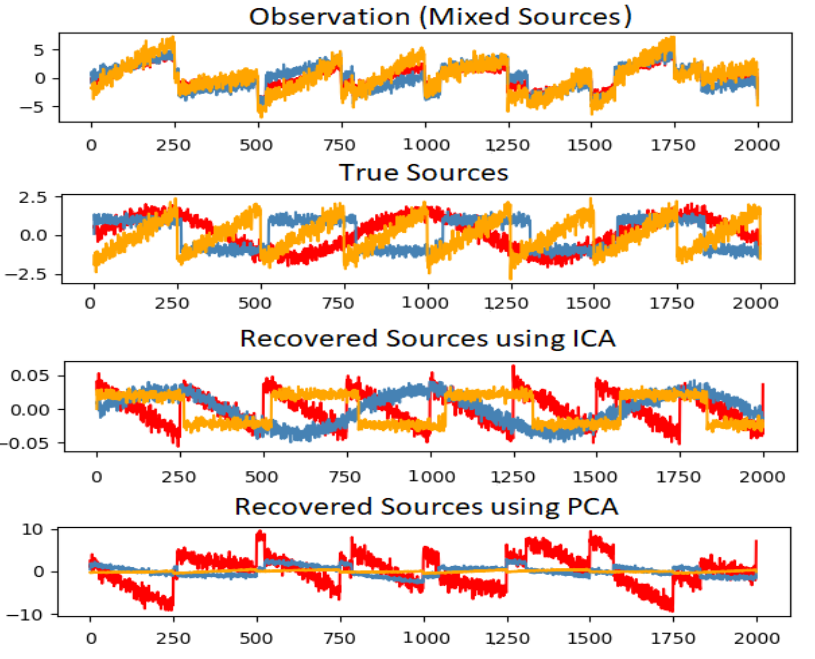
\includegraphics[scale=0.4]{img/ICA_example.png}
      \caption{We can perform this on three mixed signals with additive noise, and ICA does very well, though again some recovered signals are scaled or permuted weirdly. }
    \end{figure}
  \end{example}


\section{Slow Feature Analysis}

  Slow feature analysis also another special case of a linear factor model that uses information from time signals to learn invariant features. It is motivated by a general principle called the \textbf{slowness principle}. The idea is that the important characteristics of scenes change very slowly compared to the individual measurements that make up a description of a scene. For example, in computer vision, individual pixels can change very rapidly. If a zebra moves from left to right across the image, an individual pixel wil rapidly change from black to white. By comparison, the feature indicating whether a zebra is in the image will not change at all, and the feature describing the zebra's position will change slowly. Therefore, we want to regularize our model to learn features that change slowly over time.  

  We can apply the slowness principle to any differentiable model trained with gradient descent. That is, we can add the following term to the loss function: 
  \begin{equation}
    \lambda \sum_i d\big( f(x^{(t+1)}), f(x^{(t)}) \big)
  \end{equation}
  where $\lambda$ is a hyperparameter determining the strength of the slowness regularization term, $t$ is the time index, $f$ is the feature extractor to be regularized, and $d$ is the distance between $f(x^{(t)})$ and $f(x^{(t+1)})$. A common choice for $d$ is the mean squared difference. 

  Essentially, given a set of time-varying input signals $x^{(t)}$, SFA learns a nonlinear function $f$ that transforms $x$ into slowly-varying output signals $y$. Obviously, we can't just take some trivial function like $f = 0$, so we have the following constraints 
  \begin{align}
    \mathbb{E}_t [ f(x^{(t)})_i]  & = 0 \\ 
    \mathbb{E}_t [ f(x^{(t)})_i^2] & = 1 
  \end{align}
  \begin{center} 
    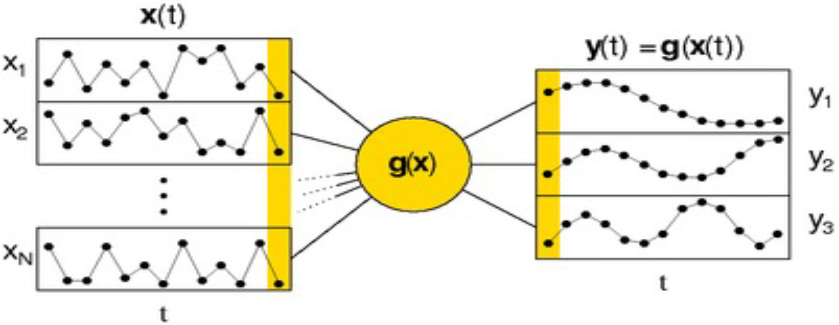
\includegraphics[scale=0.4]{img/slow_feature.png}
  \end{center}
  We can restrict the nonlinear $f$ to some subspace of functions, and this becomes a standard optimization problem where we solve 
  \begin{equation}
    \min_\theta \mathbb{E}_t \big[ \big( f(x^{(t+1)})_i - f(x^{(t)})_i \big)^2 \big]
  \end{equation}


\section{Sparse Dictionary Learning} 

  Latent variables can help us represent data in lower dimensions, but another advantage is that we can get \textit{sparse} representations as well. What we want to do in sparse coding is that for each input $x^{(i)}$, we want to find a latent representation $z^{(i)}$ such that it is sparse (i.e. has many $0$s) and also we can reconstruct the original input $x^{(i)}$ well. We have basically two things to optimize: the latent representations $z$ and the decoding mechanism, which we can do with a \textit{dictionary matrix} $D$. Note that we are optimizing for \textit{both} the latent encodings and the decoding mechanism, and so this isn't a generative model. 

  \begin{definition}[Sparse Dictionary Encoding Model]
    The \textbf{sparse dictionary encoding model} is a representation model defined 
    \begin{equation}
      X = g_{D}(Z) = D Z
    \end{equation}
    where $D \in \mathbb{R}^{d \times k}$ is a \textbf{dictionary matrix} that decodes the latent $Z \in \mathbb{R}^k$ to $X \in \mathbb{R}^d$. Note that both the $z^{(i)}$'s and $D$ are optimized, so we want to perform the \textit{joint} optimization\footnote{To break this term down, let's just assume that we have a fixed dictionary $D$. Then, we just need to minimize with respect to each $h^{(t)}$. Now we can add the dictionary parameter back again. }

    \begin{equation}
      \min_{D} \frac{1}{N} \sum_{i=1}^N \min_{z^{(i)}} \underbrace{\frac{1}{2} ||x^{(i)} - D z^{(i)}||_2^2}_{\text{reconstruction error}} + \underbrace{\lambda ||z^{(i)}||_1}_{\text{sparsity penalty}}
    \end{equation}
  \end{definition}

  Note that the reconstruction, or decoding, of $x = Dz$ is linear and explicit, but if we want to encode $x \mapsto z$, we need to substitute the $x$ into the term above and minimize it w.r.t. $D$ and $z$ to solve it. Therefore, this encoder is an implicit and \textit{nonlinear} function of $x$. 

  \begin{figure}[H]
    \centering 
    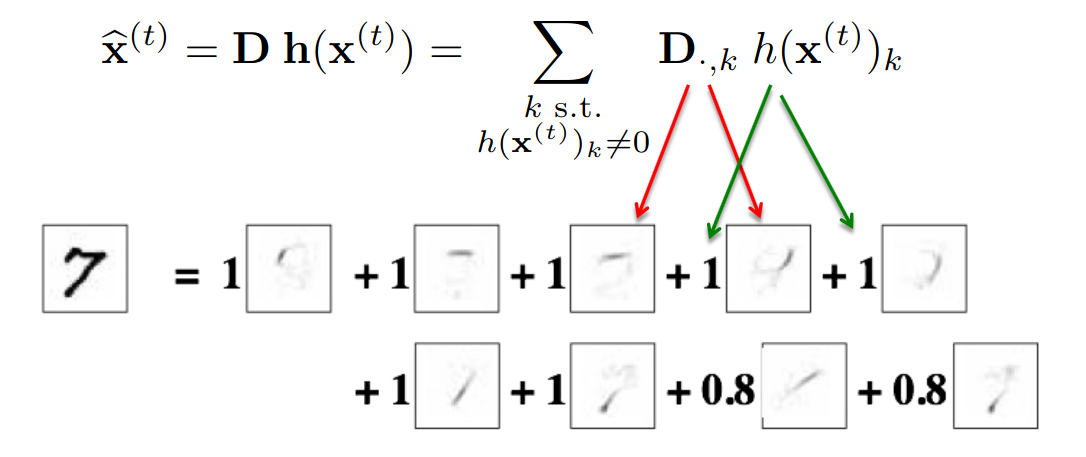
\includegraphics[scale=0.4]{img/sparse_coding.png}
    \caption{We can reconstruct an image of a seven as a linear combination of a set of images. Note that each of the images of strokes are columns of $W$ and the coefficients make up the sparse vector $h$. } 
    \label{fig:sparse_coding}
  \end{figure}

  Let's think about how we can optimize the objective function w.r.t. $h$, keeping $D$ constant. We can do stochastic gradient descent, which gives us the steps
  \begin{equation}
    \nabla_{h^{(t)}} \mathcal{L}(x^{(t)}) = D^T (D h^{(t)} - x^{(t)}) + \lambda \, \mathrm{sign}(h^{(t)})
  \end{equation}
  but this wouldn't achieve sparsity since it overshoots the $0$ all the time. Therefore, we can clip it, or we can use proximal gradient descent/ISTA to take a step, and shrink the parameters according to the L1 norm. 
  \begin{align} 
    h^{(t)} & = h^{(t)} - \alpha D^T (D h^{(t)} - x^{(t)}) \\
    h^{(t)} & = \mathrm{shrink}(h^{(t)}, \alpha \lambda)
  \end{align}
  where $\mathrm{shrink}(a, b) = [\ldots, \mathrm{sign}(a_i)\, \max(|a_i| - b_i, 0), \ldots]$. This is guaranteed to converge if $1/\alpha$ is bigger than the largest eigenvalue of $D^T D$.  



\bibliography{./bibfile}
\bibliographystyle{alpha}

\end{document}
